\documentclass[eng,printmode]{mgr}
% \documentclass[eng, printmode]{mgr}


% PREAMBULA


%% Language and font encodings
\usepackage[polish]{babel}
\usepackage[utf8x]{inputenc}
\usepackage[T1]{fontenc}

%% Sets page size and margins
\usepackage[a4paper,top=3cm,bottom=2cm,left=3cm,right=3cm,marginparwidth=1.75cm]{geometry}
%% \usepackage[a4paper, left=2.5cm, right=2.5cm, top=2.5cm, bottom=2.5cm, headsep=1.2cm]{geometry} -- Domski 

%% linki w spisie tresci, bibliografi
\usepackage[bookmarks=true,bookmarksnumbered=false,unicode=true,colorlinks=true,filecolor=black,linkcolor=black,urlcolor=black,citecolor=black]{hyperref}

\usepackage[colorinlistoftodos]{todonotes}


%OPEROWANIE NA OBRAZACH
\usepackage{graphicx}       % pakiet graficzny, umożliwiający m.in.
% import grafik w formacie eps
%\usepackage{epstopdf}		% pozwala na importowanie grafik w formacie eps
% przy użyciu pdflatex
\usepackage[update,prepend]{epstopdf}
\usepackage{rotating}       % pakiet umożliwiający obracanie rysunków
\usepackage{subfigure}      % pakiet umożliwiający tworzenie podrysunków
\usepackage{epic}           % pakiet umożliwiający rysowanie w środowisku latex
\usepackage{psfrag}         % pakiet umożliwiający podmianę łańcuchów znaków 
% w plikach eps
%\usepackage{curves}         % pakiet do wykreslania krzywych

%pakiety dodające dużo dodatkowych poleceń matematycznych
\usepackage{amsfonts}       % pakiet z rozmaitymi czcionkami matematycznymi
% \usepackage{amssymb}        % pakiet z rozmaitymi symbolami matematycznymi
\usepackage{amsmath}        % pakiet z rozmaitymi środowiskami matematycznymi

\usepackage{fp}             % pakiet z funkcjami operujacymi 
% na liczbach zmiennoprzecinkowych
\usepackage{calc}           % pakiet umożliwiający operacje arytmetyczne
% na tzw. licznikach (liczbach całkowitych)
\usepackage{leftidx}		% indeksy górne i dolne po lewej stronie

%definicje matematyczne
\providecommand{\abs}[1]{\lvert#1\rvert}
\providecommand{\norm}[1]{\lVert#1\rVert}

%pakiety wspomagające i poprawiające składanie tabel
\usepackage{supertabular}
\usepackage{array}
\usepackage{tabularx}
\usepackage{hhline}
\usepackage{longtable}		% wsparcie dla dlugich tabel
\usepackage{multicol}		% podzial strony na wiele kolumn

%pakiet do BibTex
\usepackage{cite}

\usepackage{url} %pakiet pozawalający na dodawanie adresów url w bibliografi

%pakiet wypisujący na marginesie etykiety równań i rysunków zdefiniowanych przez \label{}, chcąc wygenerować finalną wersję dokumentu wystarczy usunąć poniższą linię
%\usepackage{showlabels}

\usepackage{float}			% lepsza obsluga mechanizmow obiektow plywajacych
% wymuszenie wstawienia np. tabeli, obrazka w danym miejscu przez [H]

\usepackage{listings}       % pakiet dedykowany zrodlom programow
\usepackage{color}


\definecolor{dkgreen}{rgb}{0,0.6,0}
\definecolor{gray}{rgb}{0.5,0.5,0.5}
\definecolor{mauve}{rgb}{0.58,0,0.82}

\lstset{ %
	language=Matlab,                % the language of the code
	basicstyle=\scriptsize,           % the size of the fonts that are used for the code
	numbers=left,                   % where to put the line-numbers
	numberstyle=\tiny\color{gray},  % the style that is used for the line-numbers
	stepnumber=1,                   % the step between two line-numbers. If it's 1, each line 
	% will be numbered
	numbersep=5pt,                  % how far the line-numbers are from the code
	backgroundcolor=\color{white},      % choose the background color. You must add \usepackage{color}
	showspaces=false,               % show spaces adding particular underscores
	showstringspaces=false,         % underline spaces within strings
	showtabs=false,                 % show tabs within strings adding particular underscores
	%frame=single,                   % adds a frame around the code
	rulecolor=\color{black},        % if not set, the frame-color may be changed on line-breaks within not-black text (e.g. comments (green here))
	tabsize=2,                      % sets default tabsize to 2 spaces
	captionpos=b,                   % sets the caption-position to bottom
	breaklines=true,                % sets automatic line breaking
	breakatwhitespace=false,        % sets if automatic breaks should only happen at whitespace
	%title=\lstname,                   % show the filename of files included with \lstinputlisting;
	% also try caption instead of title
	keywordstyle=\color{blue},          % keyword style
	commentstyle=\color{dkgreen},       % comment style
	stringstyle=\color{mauve},         % string literal style
	escapeinside={\%*}{*)},            % if you want to add LaTeX within your code
	morekeywords={*,...},              % if you want to add more keywords to the set
	deletekeywords={...}              % if you want to delete keywords from the given language
}

%polish signs in lst code
\lstset{literate=%
	{ą}{{\k{a}}}1
	{ć}{{\'c}}1
	{ę}{{\k{e}}}1
	{ł}{{\l}}1
	{ń}{{\'n}}1
	{ó}{{\'o}}1
	{ś}{{\'s}}1
	{ż}{{\.z}}1
	{ź}{{\'z}}1
	{Ą}{{\k{A}}}1
	{Ć}{{\'C}}1
	{Ę}{{\k{E}}}1
	{Ł}{{\L}}1
	{Ń}{{\'N}}1
	{Ó}{{\'O}}1
	{Ś}{{\'S}}1
	{Ż}{{\.Z}}1
	{Ź}{{\'Z}}1
}

\usepackage{verbatim}       % pakiet dedykowany rozmaitym wydrukom tekstowym
\usepackage{ifthen}         % pakiet umożliwiający tworzenie prostych programów
% (m.in. zawiera instrukcje powtórzeniowe 
% i warunkowe)
\usepackage{upquote}		%normal quotations marks ' and `

% deklaracje wymagane przez pakiet theorem automatycznie ladowany w przypadku
% klasy dokumentu article
%
\newtheorem{Dn}{Definicja}[section]     % deklaracja srodowiska definicja
\newtheorem{La}[Dn]{Lemat}                % deklaracja srodowiska lemat
\newtheorem{Tm}[Dn]{Twierdzenie}          % deklaracja srodowiska twierdzenie
\newtheorem{Rk}[Dn]{Spostrze{\.z}enie}  % deklaracja srodowiska spostrzezenie
\newtheorem{Am}[Dn]{Algorytm}           % deklaracja srodowiska algorytm
\newtheorem{As}[Dn]{Za{\l}o{\.z}enie}   % deklaracja srodowiska zalozenie
\newtheorem{Pn}[Dn]{Propozycja}           % deklaracja srodowiska propozycja
\newtheorem{Py}[Dn]{W{\l}asno{\'s}{\'c}}  % deklaracja srodowiska wlasnosc
\newtheorem{Cy}[Dn]{Wniosek}              % deklaracja srodowiska wniosek
\newtheorem{Ee}[Dn]{Przyk{\l}ad}        % deklaracja srodowiska przyklad
\newtheorem{Ex}{{\'C}wiczenie}          % deklaracja srodowiska cwiczenie

\newtheorem{theorem}{Twierdzenie}[section] %nowe otoczenie do składania twierdzeń
%definicje własnych poleceń
\newcommand{\R}{I\!\!R} %symbol liczb rzeczywistych, działa tylko w trybie matematycznym

%helps to specify width of a column in table
%\begin{tabular}{|C{1cm}|c|c|c|c|c|c|c|c|c|c|}
%first column will have widht of 1cm
\newcolumntype{L}[1]{>{\raggedright\let\newline\\\arraybackslash\hspace{0pt}}m{#1}}
\newcolumntype{C}[1]{>{\centering\let\newline\\\arraybackslash\hspace{0pt}}m{#1}}
\newcolumntype{R}[1]{>{\raggedleft\let\newline\\\arraybackslash\hspace{0pt}}m{#1}}

\sloppy			%zawija bardzo długie linie

%\pagenumbering{gobble}% Remove page numbers (and reset to 1)

% \include{bibliografia}


%pakiety do grafiki
\usepackage{graphicx}


% re-definiowane polecenie w celu przechowywania nazwiska autora, jego brak powoduje ostrzezenie (Warning) podczas przetwarzania.
\author{Wojciech Kosicki} 

% re-definiowane polecenie w celu przechowywania polskiego tytułu pracy magisterskiej, jego brak powoduje ostrzezenie (Warning) podczas przetwarzania.
\title{Parametryzacja nieortogonalna 3D w zadaniu śledzenia ścieżek robotów} 


% polecenie zdefiniowane w celu przechowywania angielskiego tytułu pracy magisterskiej, jego brak powoduje ostrzezenie (Warning) podczas przetwarzania.
\engtitle{Non-orthogonal 3D parametrization in path following task of robots} 


% polecenie zdefiniowane w celu przechowywania danych osobowych prowadzacego prace, jego brak powoduje ostrzezenie (Warning) podczas przetwarzania.
\supervisor{Dr hab. inż. Alicja Mazur, Prof. PWr K7/W4} 




% polecenie zdefiniowane w celu przechowywania nazwy kierunku studiów, jego brak powoduje ostrzezenie (Warning) podczas przetwarzania.
\field{Automatyka i Robotyka (AIR)} 

%\specialisation{Robotyka}


% re-definiowane polecenie w celu przechowywania roku. Standardowo u dołu strony tytułowej wstawiany jest biezacy rok, uzycie tego polecenia pozwala wstawic dowolny rok.
\date{2018} 



\begin{document}
\maketitle


\tableofcontents
% \listoffigures
% \listoftables



\chapter{Wstęp}


Rewolucja przemysłowa, która rozpoczęła się w Anglii,  drastycznie zmieniła świat w XIX wieku. Pomimo jednak rozwinięcia gospodarki oraz opracowania wielu technologii, do drugiej połowy XX wieku główną siłą roboczą byli tani pracownicy. Powojenny świat wymagał szybkiej odbudowy przemysłu i powstało wielkie zapotrzebowanie na usprawnienie linii produkcyjnych. Zaczęły powstawać pierwsze roboty przemysłowe. Roboty te zaczęły powoli zastępować ludzi przy liniach produkcyjnych. Były szybsze od człowieka i mogły pracować znacznie dłużej. Na przestrzeni kolejnych sześćdziesięciu lat rozwoju tej dziedziny, powstało wiele rodzajów i modelów manipulatorów do różnych prac w fabrykach. Jednak większość manipulatorów jest zbudowana z przegubów obrotowych. Wynika to z faktu, że przeguby przesuwne są trudne do wykonania oraz sterowania. Takie roboty miały ograniczone bardzo możliwości. Nie mogły poruszać swoim efektorem po liniach prostych, dlatego też nie mogły wykonywać wielu prostych czynności m.in. dokonać spawania po linii prostej. Dopiero zastosowanie po wielu latach algorytmu odsprzęgania wejściowo-wyjściowego umożliwiło sterowanie efektorem po odcinkach prostych w manipulatorach z przegubami obrotowymi. 
\section{Cel pracy}
Celem pracy jest zapoznanie się z algorytmem odpsrzęgania wejściowo-wyjściowego do sterowania manipulatorem IRb-6. Dzięki temu algorytmowi będzie możliwe sterowanie efektorem manipulatora po liniach prostych, pomimo tego, że robot posiada pięć obrotowych stopni swobody.
\section{Zawartość pracy}
Rozdział pierwszy zawiera wstęp oraz opis celu pracy. W rozdziale drugim omówiono modelowanie manipulatora IRb-6 w środowisku Matlab/Simulink. Opisano jego dynamikę oraz kinematykę. Rozdział trzeci dotyczy algorytmu odsprzęgania wejściowo-wyjściowego oraz jego implementacji. W tym rozdziale zawarto także opis konfiguracji osobliwych manipulatora. W rozdziale czwartym zawarto model generatora trajektorii zadanej dla efektora oraz regulację PD z korekcją. Przeprowadzono też badania symulacyjne działania całego układu. W ostatnim, piąty, rozdziale dokonano podsumowania pracy.
\newpage
\chapter{Modelowanie manipulatora IRb-6}

\section{Zasada Najmniejszego Działania}



Aby zdefiniować równania robota, należy najpierw wyprowadzić tzw. lagranżian układu
\begin{equation}\label{row2.1}
L(q,\dot{q})=K(q,\dot{q})-V(q)=\frac{1}{2}\dot{q}^TM(q)\dot{q}-V(q).
\end{equation}
Zmienne $q ∈ R^3$ określają wektor położeń przegubów robota, zaś  $\dot{q} ∈ R^3 $ określają prędkości IRb-6. Zmienne te składają się na stan modelowanego układu. Lagranżian jest różnicą energii kinetycznej $K(q,\dot{q})$ oraz potencjalnej $V(q)$. Zgodnie z Zasadą Najmniejszego Działania, lagranżian musi spełniać równanie Eulera-Langrange'a, czyli
\begin{equation}\label{row2.2}
\frac{d}{dt}  \frac{∂L(q,\dot{q})}{∂\dot{q}} - \frac{∂L(q,\dot{q})}{∂q}=F_{zew}.
\end{equation}
$F_{zew}$ to siła wypadkowa oddziaływań zewnętrznych na układ. Uwzględnia ona siły oraz momenty sił wpływające na układ, m.in. siły oporu ruchu, siły tarcia czy siły sterujące manipulatorem. Składowa ta będzie oznaczana jako sygnał sterujący $u$. Podstawiając (\ref{row2.1}) do (\ref{row2.2}), otrzymuje się równanie dynamiki w postaci
\begin{equation}\label{row2.3}
 \frac{∂^2L(q,\dot{q})}{∂\dot{q}^2}\ddot{q} +\frac{∂^2L(q,\dot{q})}{∂q∂\dot{q}}\dot{q} - \frac{∂L(q,\dot{q})}{∂q}=u.
\end{equation}
 Uwzględniając postać energii kinetycznej robota daną wzorem (\ref{row2.1}), w postaci formy kwadratowej, uzyskano następujące równania dynamiki robota
\begin{equation}\label{row2.4}
M(q)\ddot{q}+C(q, \dot{q})\dot{q} + D(q)=u.
\end{equation}


Macierz $M(q)$ jest tzw. macierzą bezwładności, która jest symetryczna i dodatnio określona. Jest to macierz formy pojawiająca się w energii kinetycznej. Z kolei $C(q,\dot{q})$  to macierz sił Coriolisa oraz sił odśrodkowych. Trzeci element modelu, $D(q)$, to wektor opisujący siły oddziaływania grawitacyjnego na układ. 
\newpage
\section{Dynamika manipulatora IRb-6}
Założono, że model IRb-6 jest manipulatorem sztywnym. Założenie takie uwzględnia nieruchomość bazy manipulatora oraz fakt, że ramię IRb-6 składa się ze sztywnych ogniw połączonych przegubami sztywnymi. \newline


Robot IRb-6 posiada pięć stopni swobody, jednak czwarty i piąty stopień są odpowiedzialne jedynie za orientację manipulatora, można więc je zignorować przy opisywaniu pozycji chwytaka. Przy takim założeniu można potraktować IRb-6 jako manipulator z trzema stopniami swobody.

Pierwszym krokiem w tworzeniu modelu robota IRb-6 będzie opracowanie jego dynamiki. W tym celu wykorzystane zostaną wcześniejsze równania (\ref{row2.4}).
Modelowanie i badania będą przeprowadzone w środowisku Matlab/Simulink, jednak należy pamiętać, że pakiet Matlab rozwiązuje równania różniczkowe w sposób numeryczny. Aby móc go zastosować, należy najpierw przekształcić równania (\ref{row2.4}) do takiej postaci, które umożliwią rozwiązanie ich tą metodą. W tym celu należy przedstawić dynamikę w postaci $\ddot{q}=f(\dot{q}, q)$. Przekształcając kolejno
\begin{equation}
M(q)\ddot{q}=u - C(q, \dot{q})\dot{q} - D(q),\label{row2.7}
\end{equation}
a następnie mnożąc równanie lewostronnie przez $M^{-1}(q)$, otrzymuje się wzór
\begin{equation}
\ddot{q} = M^{-1}(q) (u - C(q, \dot{q})\dot{q} - D(q)),\label{row2.8}
\end{equation}
lub równoważnie
\begin{equation}\label{row2.9}
\ddot{q} = F(q) (u - C(q, \dot{q})\dot{q} - D(q)),
\end{equation}
gdzie 
\begin{equation}
F(q)=M^{-1}(q) .
\end{equation}
Macierz $F(q)$  jest odwrotnością macierzy bezwładności $M(q)$, której postać dla manipulatora IRb-6 jest następująca
\begin{eqnarray}\label{row2.11}
M(q)=\left[
        \begin{array}{ccc}
         M_{11}& 0 & 0\\ 
         0 & M_{22} & M_{23}\\
         0 & M_{23} & M_{33}
         \end{array}
      \right].
\end{eqnarray}
Poszczególne elementy tej macierzy są równe
\begin{eqnarray}\label{row2.12}
M_{11} &=& 5.66+6.56125s_2^2  -0.531s_2c_3 + 10.9c_3^2,\\
M_{22} &=& 11.18525,\nonumber \\
M_{23} &=& 0.13275s_{23},\nonumber \\
M_{33} &=& 15.524.\nonumber
\end{eqnarray}
 gdzie $c_i$, $s_i$ to oznaczenia dla $\cos(q_i)$ oraz $\sin(q_i)$, natomiast $s_{23}=\sin(q_2+q_3)$.

Macierz $F(q)$ będąca odwrotnością macierzy $M(q)$ jest wyliczana z definicji jako
\begin{equation}\label{row2.13}
F(q)=M(q)^{-1}=\frac{1}{detM(q)} \cdot (M(q)^d)^T,
\end{equation}
gdzie $detM(q)$ to wyznacznik macierzy $M(q)$, a $M(q)^d$ to macierz dopełnień algebraicznych dla macierzy bezwładności. Pojawia się tu pewne ułatwienie, albowiem macierz dopełnienia jest macierzą symetryczną
\begin{equation}
(M(q)^d)^T = M(q)^d.
\end{equation}
Dzięki temu, można uprościć zależność do postaci
\begin{equation}
F(q)=M(q)^{-1}=\frac{1}{detM(q)} \cdot M(q)^d.
\end{equation}
Wyznacznik macierzy bezwładności (\ref{row2.11}) jest równy
\begin{eqnarray}
detM(q)= (5.66+6.56125s_2^2 - 0.531s_2c_3 + 10.9c_3^2)\nonumber \\
(173.639821 - (0.13275s_{23})^2.
\end{eqnarray}
Wykorzystując oznaczenia (\ref{row2.12}) wyznacznik ten można zapisać inaczej
\begin{equation}\label{row2.17}
detM(q)= M_{11} \cdot (M_{22} \cdot M_{33} - (M_{23})^2).
\end{equation}
Kolejnym krokiem było wyliczenie macierzy dopełnienia $M(q)^d$ 
\begin{eqnarray}\label{row2.18}
M(q)^d=\left[
        \begin{array}{ccc}
         M_{22} \cdot M_{33} - (M_{23})^2 & 0 & 0\\ 
         0 & M_{11}M_{33} & -M_{11}M_{23}\\
         0 & -M_{11}M_{23} & M_{11}M_{22}
         \end{array}
      \right] 
\end{eqnarray}
Dokonano wyliczenia macierzy odwrotnej jako
\begin{eqnarray}
M(q)^{-1}= \frac{1}{M_{11} \cdot (M_{22} \cdot M_{33} - (M_{23})^2)} \cdot \left[
        \begin{array}{ccc}
         M_{22} \cdot M_{33} - (M_{23})^2 & 0 & 0\\ 
         0 & M_{11}M_{33} & -M_{11}M_{23}\\
         0 & -M_{11}M_{23} & M_{11}M_{22}
         \end{array}
      \right].\nonumber
      \end{eqnarray}
      Po odpowiednim wymnożeniu uzyskano
 \begin{eqnarray}
F(q)=M(q)^{-1}= \left[
        \begin{array}{ccc}
         F_{11} & 0 & 0\\ 
         0 & F_{22}  & F_{23}\\
         0 & F_{23}  & F_{33}
         \end{array}
      \right].
\end{eqnarray}
gdzie
\begin{eqnarray}\label{row2.20}
F_{11} &= &\frac{1}{M_{11}},\\
F_{22} &= &\frac{M_{33}}{M_{22} \cdot M_{33} - (M_{23})^2},\nonumber \\
F_{23} &= &\frac{-M_{23}}{M_{22} \cdot M_{33} - (M_{23})^2},\nonumber \\
F_{33} &= &\frac{M_{22}}{M_{22} \cdot M_{33} - (M_{23})^2}.\nonumber
\end{eqnarray}


Teraz, znając odpowiednie funkcje, można zaimplementować macierz $M(q)$ oraz $F(q)$ w środowisku Simulink. Należy jednak pamiętać, że Matlab liczy równanie różniczkowe metodą numeryczną. Najpierw więc stworzono układ, który generuje zmienne stanu $q$ oraz $\dot{q}$.
  
  
Bloki odpowiedzialne za przeliczenie macierzy $M(q)$ oraz $F(q)$ zawarto w bloku dynamiki w programie Simulink.
Następnym blokiem, jaki należy opracować, jest blok odpowiedzialny za macierz sił odśrodkowych i sił Coriolisa, $C(q, \dot{q})$. Wykorzystując dane z pracy \cite{b4}, przyjęto następującą postać tej macierzy
 \begin{eqnarray}
 C(q, \dot{q})=  \left[
        \begin{array}{ccc}
         C_{12}^*\dot{q}_2+C_{13}^*\dot{q}_3 & C_{12}^*\dot{q}_1 & C_{13}^*\dot{q}_1\\ 
         -C_{12}^*\dot{q}_1 & 0 & 2C_{23}^*\dot{q}_2+C_{33}^*\dot{q}_3\\
         -C_{13}^*\dot{q}_1 & -C_{23}^*\dot{q}_2 & 0
         \end{array}
      \right],
 \end{eqnarray}
 gdzie
  \begin{eqnarray}
C_{12}^* &=& \frac{1}{2}(6.56125s_{22}-0.531c_2c_3),\nonumber\\
C_{13}^* &=& -\frac{1}{2}(-0.531s_2s_3+10.9s_{33}),\nonumber  \\
C_{23}^* &=& 0.13275c_{23}, \nonumber\\
C_{33}^* &=& 0.13275c_{23} . \end{eqnarray}
   Macierz ta została uproszczona do postaci
  \begin{eqnarray}
C(q, \dot{q})=  \left[
        \begin{array}{ccc}
         C_{11} & C_{12} & C_{13}\\ 
         -C_{12} & 0 & C_{23}\\
         -C_{13} & C_{32} & 0
         \end{array}
      \right],
 \end{eqnarray}
 gdzie \\
 \begin{eqnarray}
C_{11} &=& \frac{1}{2}\dot{q}_2(6.56125s_{22}-0.531c_2c_3)\nonumber\\
&-&\frac{1}{2}\dot{q}_3(-0.531s_2s_3+10.9s_{33}), \nonumber\\
C_{12} &=& \frac{1}{2}\dot{q}_1(6.56125\sin(2q_2)-0.531c_2c_3), \nonumber  \\
C_{13} &=& -\frac{1}{2}\dot{q}_1(-0.531s_2s_3+10.9\sin(2q_3)), \nonumber \\
C_{23} &=& 0.2655c_{23}(\dot{q}_2+\frac{1}{2}\dot{q}_3), \nonumber \\
C_{32} &=& 0.13275\dot{q}_2c_{23}.\nonumber\\
\end{eqnarray}
Wektor oddziaływań grawitacyjnych $D(q)$ ma prostą strukturę
\begin{eqnarray}
D(q)=  \left[
        \begin{array}{c}
         D_1\\ 
        D_2\\
         D_3
         \end{array}
      \right],
\end{eqnarray}
 gdzie
 \begin{eqnarray}
D_1 &=& 0, \nonumber\\
D_2 &=& -145\sin(q_2), \nonumber\\
D_3 &=& -5.7879\cos(q_3) . \nonumber\\
\end{eqnarray}


Punktem wyjściowym do implementacji dynamiki w Matlabie było równanie (\ref{row2.9}).
W pełnej swojej postaci wygląda ono następująco
  \begin{eqnarray}
 \left[
        \begin{array}{c}
         \ddot{q}_1\\ 
        \ddot{q}_2\\
         \ddot{q}_3
         \end{array}
      \right]=\left[
        \begin{array}{ccc}
         F_{11} & 0 & 0\\ 
         0 & F_{22}  & F_{23}\\
         0 & F_{23}  & F_{33}
         \end{array}
      \right]\left(\left[
      \begin{array}{c}
         u_1\\ 
        u_2\\
         u_3
         \end{array}
      \right]-\left[
      \begin{array}{ccc}
         C_{11} & C_{12} & C_{13}\\ 
         -C_{12} & 0 & C_{23}\\
         -C_{13} & C_{32} & 0
         \end{array}
      \right]\left[
        \begin{array}{c}
         \dot{q}_1\\ 
        \dot{q}_2\\
         \dot{q}_3
         \end{array}
      \right]-\left[
        \begin{array}{c}
         D_1\\ 
        D_2\\
         D_3
         \end{array}
      \right]
      \right).   
 \end{eqnarray}
 Po dokonaniu odpowiednich działań na macierzach w nawiasie uzyskano wyrażenie
\begin{eqnarray}
 \left[
        \begin{array}{c}
         \ddot{q}_1\\ 
        \ddot{q}_2\\
         \ddot{q}_3
         \end{array}
      \right]=\left[
        \begin{array}{ccc}
         F_{11} & 0 & 0\\ 
         0 & F_{22}  & F_{23}\\
         0 & F_{23}  & F_{33}
         \end{array}
      \right]\left[
        \begin{array}{c}
         h_1\\ 
        h_2\\
         h_3
         \end{array}
      \right],
     \end{eqnarray}
gdzie\\
\begin{eqnarray}
h_1 &=& u_1 - C_{11}\dot{q}_1 - C_{12}\dot{q}_2 - C_{13}\dot{q}_3 - D_1 ,\nonumber\\
h_2 &=& u_2 + C_{12}\dot{q}_1 - C_{23}\dot{q}_3 - D_2,\nonumber\\
h_3 &=&u_3 + C_{13}\dot{q}_1 - C_{32}\dot{q}_2 - D_3 .
 \end{eqnarray}
 
 
W ten sposób można zaimplementować nie tylko bloki $C(q, \dot{q})$, $D(q)$, ale także wyprowadzenie sygnału $\ddot{q}∈ R^3 $.  
Na końcu implementacji tego bloku trzeba połączyć układ z sygnałem sterującym $u ∈ R^3 $. Ostateczny kształt układu dynamiki w programie Simulink został zamieszczony poniżej.
\begin{figure}[!ht]
\centering
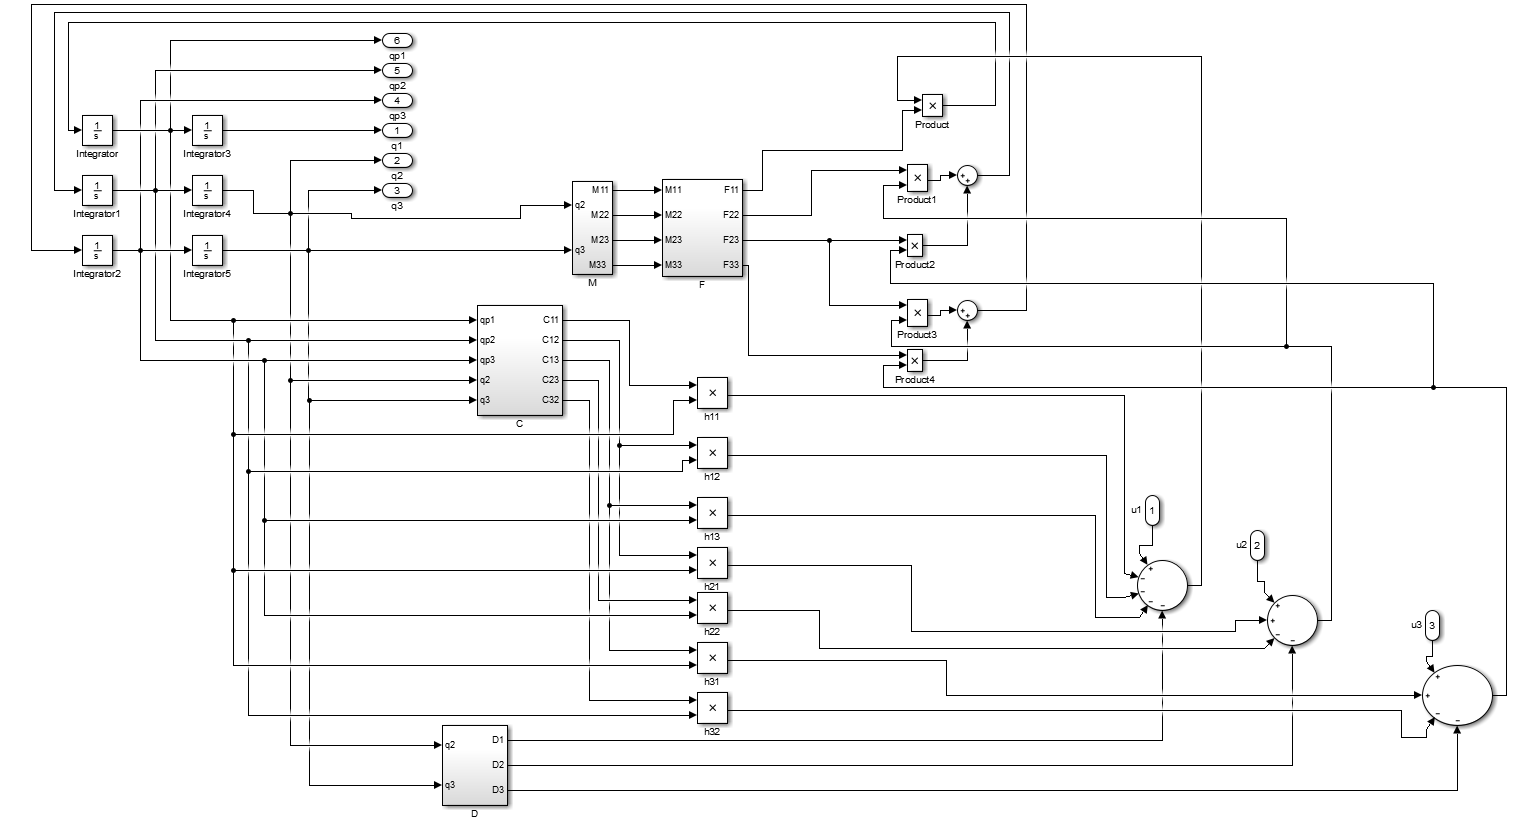
\includegraphics[width=1\textwidth]{02.png}
\caption{\label{fig:blok5}Dynamika manipulatora IRb-6 w programie Simulink.}
\end{figure}
\newpage
\section{Kinematyka manipulatora IRb-6 według Denavita-Hartenberga}
W celu stworzenia kompletnego opisu matematycznego manipulatora IRb-6, oprócz jego dynamiki należy także określić jego kinematykę. Została ona opisana przy użyciu notacji Denavita-Hartenberga. Notacja ta pozwala opisać kinematykę robotów będących ramionami mechanicznymi według międzynarodowych standardów. 


Parametry $d_1, d_6, a_2, a_3$ wynikają z własności fizycznych badanego manipulatora. Wynoszą one odpowiednio:\\
$d_1 = 0.7$ $[m]$,\\
$d_6 = 0.095$ $[m]$,\\
$a_2 = 0.45$ $[m]$,\\
$a_3 = 0.67$ $[m]$.\\


Manipulator IRb-6 ma pięć stopni swobody, jednak na jego położenie kąty $q_4$ oraz $q_5$ nie będą miały wpływu. Wynika to z faktu, że zmienne te są odpowiedzialne jedynie za obrót samego chwytaka. Można dzięki temu całą notację przedstawić jako odwzorowania
\begin{equation}
\textbf{K(q)}= {A_0}^1{A_1}^2{A_2}^3{A_3}^4{A_4}^5(q):X_0Y_0Z_0 \to X_5Y_5Z_5
\end{equation}
gdzie\\
${A_0}^1=\textbf{Rot}(Z, q_1)\textbf{Trans}(Z, d_1)\textbf{Rot}(X,\frac{\pi}{2})$,\\
${A_1}^2=\textbf{Rot}(Z, q_2)\textbf{Trans}(Z, a_2)$,\\
${A_2}^3=\textbf{Rot}(Z, q_3-q_2)\textbf{Trans}(X, a_3)$,\\
${A_3}^4=\textbf{Rot}(Z, q_4-q_3)\textbf{Rot}(X, \frac{\pi}{2})$,\\
${A_4}^5=\textbf{Rot}(Z, q_5)\textbf{Trans}(Z, d_6)\textbf{Rot}(X, -\frac{\pi}{2})$.\\
Po przemnożeniu w odpowiedniej kolejności tych odwzorowań wyliczono macierz kinematyki jako
\begin{eqnarray}
\textbf{K(q)}= \left[
        \begin{array}{cccc}
         c_1c_4c_5+s_1s_5 & -c_1s_4 &s_1c_5 -c_1c_4s_5 & c_1(a_2c_2+a_3c_3+d_6s_4)\\ 
       -s_4c_5& -c_4& s_4s_5& -d_1+d_6c_4-a_2s_2-a_3s_3\\
         s_1c_4c_5-c_1s_5& -s_1s_4& -c_1c_5-s_1c_4s_5& s_1(a_2c_2+a_3c_3+d_6s_4)\\
         0&0&0&1
         \end{array}
      \right],
\end{eqnarray} 
     
Trzy pierwsze elementy z ostatniej kolumny tej macierzy decydują o współrzędnych lokalizacji efektora w przestrzeni roboczej. Dlatego potrzebny do określenia kinematyki układ równań ma postać

\begin{eqnarray}
\left\{ \begin{array}{lll}
x&=& c_1(a_2c_2+a_3c_3+d_6s_4)\\ 
y&=&-d_1+d_6c_4-a_2s_2-a_3s_3\\ 
z&=&s_1(a_2c_2+a_3c_3+d_6s_4)  \label{row2.30}
\end{array} \right.
\end{eqnarray}




Jak widać, położenie chwytaka zależy od położenia przegubów $q_1 \div q_4$. Pozycje przegubów $q_1\div q_3$ otrzymuje się z dynamiki robota, natomiast kąt $q_4$, który jest potrzebny do wyliczenia położenia chwytaka, ma stałą wartość, ustalaną przez operatora. Z kolei $q_5$ wpływa tylko na orientację IRb-6, a nie na położenie chwytaka.  Dlatego też przyjęto, że wartość kąta $q_5$ będzie ustaloną wartością stałą.


Na podstawie tych równań dokonano implementacji kinematyki robota IRb-6 w programie Simulink. Równania zarówno dynamiki i kinematyki takiego układu mają postać
\begin{eqnarray}
&M(q)\ddot{q}+C(q, \dot{q})\dot{q} + D(q)=u ,\label{row2.5}\\
&y=K(q). \label{row2.6}
\end{eqnarray}
Powyższy opis dynamiki i kinematyki układu będzie podstawą do zamodelowania robota IRb-6 w programie Simulink.
Sygnał wejściowy to $u ∈ R^3$, a współrzędne położenia efektora manipulatora to $x, y, z$. Wartości $qp1, qp2, qp3$ to odpowiednio $\dot{q}_1, \dot{q}_2, \dot{q}_3$. 
\begin{figure}[!ht]
\centering
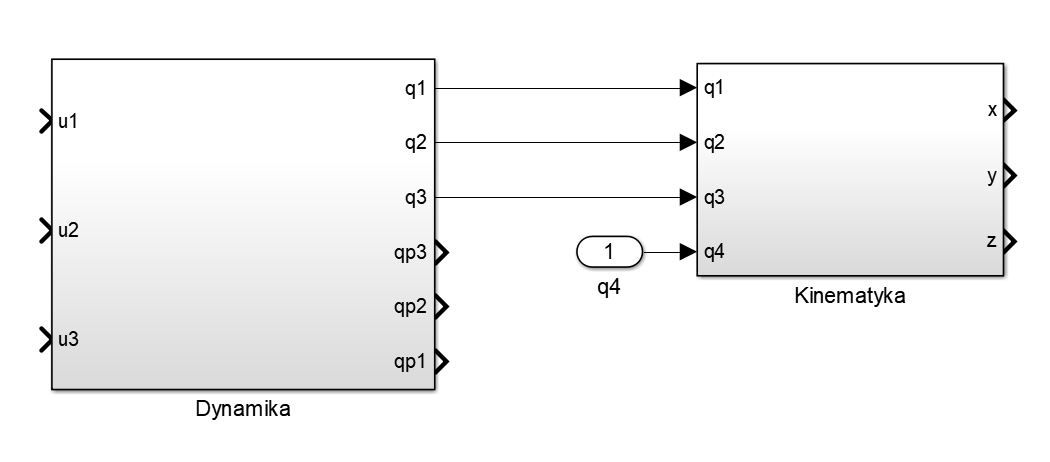
\includegraphics[width=1.1\textwidth]{01.png}
\caption{\label{fig:blok1}Bloki dynamiki i kinematyki IRb-6 w programie Simulink.}
\label{rys1}
\end{figure}
\chapter{Algorytm odsprzęgania wejściowo-wyjściowego}
\section{Afiniczny układ sterowania}
Po zaimplementowaniu modelu manipulatora w programie symulacyjnym, można przystąpić do opracowania algorytmu odsprzęgania wejściowo-wyjściowego. Algorytm odsprzęgania wejściowo-wyjściowego składa się z dwóch części: odsprzężenia i linearyzacji przekształcenia wejściowo-wyjściowego oraz sterowania dla odsprzężonego układu liniowego. Taki algorytm pozwoli użytkownikowi sterować manipulatorem IRb-6 w sposób liniowy, tak jakby robot posiadał przeguby przesuwne.


Najpierw należy zacząć od uzyskania afinicznego układu sterowania. 
W poprzednim rozdziale zostały określone równania opisujące dynamikę i kinematykę manipulatora (\ref{row2.5}), ({\ref{row2.6}).
Drugie równanie opisuje kinematykę układu.
\begin{equation}\label{row3.1}
y_{CHi}=k_i(q),\ \ i=1,...,p,
\end{equation}
które w postaci wektorowej wygląda następująco
\begin{eqnarray}
 y_{CH}=\left[
        \begin{array}{c}
         k_1\\ 
        k_2\\
         k_3
         \end{array}
      \right]=\left[
        \begin{array}{c}
         x\\ 
        y\\
        z
         \end{array}
      \right].
\end{eqnarray}


Jak widać, dla robota IRb-6 liczba wyjść jest równa $p=3$.
W celu uzyskania postaci afinicznej, należy uzyskać pochodną drugiego rzędu równania (\ref{row3.1}) po czasie. Dlatego zostaną wyliczone pochodne dla każdej składowej wektora $k(q)$ 
\begin{equation}
\frac{d}{dt}y_{CHi}=\frac{d}{dt}k_i(q)=\frac{∂k_i}{∂q}\frac{dq}{dt}=\frac{∂k_i}{∂q}\dot{q},\ \ i=1,...,p.
\end{equation}
\\Dla całego wektora pochodna będzie wynosiła zatem
\begin{equation}
\dot{y}_{CHi}=\frac{∂k_i}{∂q}\dot{q},\ \ i=1,...,p,
\end{equation}
a dla pochodnej drugiego rzędu zachodzi
\begin{equation}\label{row3.5}
\ddot{y}_{CHi}=\frac{d}{dt}\left(\frac{∂k_i}{∂q}\right)\dot{q}+\frac{∂k_i}{∂q}\ddot{q}=\dot{q}^T\frac{∂^2k_i}{∂q^2}\dot{q}+\frac{∂k_i}{∂q}\ddot{q},\ \ i=1,...,p.
\end{equation}
Należy zwrócić uwagę na iloczyn $\dot{q}^T\frac{∂^2k_i}{∂q^2}\dot{q}$. Nie jest on macierzą, tylko skalarem, który oznaczony zostanie jako $P_i$. Równanie (\ref{row3.5}) można zatem uprościć do postaci
\begin{equation}\label{row3.6}
\ddot{y}_{CHi}= P_i +\frac{∂k_i}{∂q}\ddot{q},\ \ i=1,...,p.
\end{equation}
Równanie (\ref{row3.6}) dotyczy wszystkich składowych pozycji chwytaka, czyli zachodzi
\begin{equation}\label{row3.7}
\ddot{y}_{CH}=\left[
        \begin{array}{c}
         \ddot{x}\\ 
       \ddot{y}\\
         \ddot{z}
         \end{array}
      \right]=\left[
        \begin{array}{c}
         P_1\\ 
        P_2\\
        P_3
         \end{array}
      \right]+\left[
        \begin{array}{c}
         \frac{∂k_1}{∂q}\\ 
      \frac{∂k_2}{∂q}\\
         \frac{∂k_3}{∂q}
         \end{array}
      \right]\ddot{q}= P+J\ddot{q}.
\end{equation}
Symbol $J$ oznacza macierz Jacobiego. kinematyki (\ref{row2.30}) wynosi

\large{\begin{eqnarray}
J=\left[
      \begin{array}{ccc}
         \frac{∂k_1}{∂q_1} & \frac{∂k_1}{∂q_2} & \frac{∂k_1}{∂q_3}\\ 
         &&\\
         \frac{∂k_2}{∂q_1} & \frac{∂k_2}{∂q_2} & \frac{∂k_2}{∂q_3}\\
         &&\\
         \frac{∂k_3}{∂q_1} & \frac{∂k_3}{∂q_2} & \frac{∂k_3}{∂q_3}
         \end{array}
      \right].\nonumber
\end{eqnarray}}}
      Kolejnym krokiem jest podstawienie równań dynamiki do  układu (\ref{row3.7}). Wyliczoną wartość $\ddot{q}$ podstawia się do równania (\ref{row3.7}), otrzymując
     \begin{equation}
\ddot{y}_{CH}= P +JF(q)(u - C(q, \dot{q})\dot{q} - D(q))=P+JF(q)u-JF(q)(C(q, \dot{q})\dot{q} + D(q)).
\end{equation} 
Z powyższego równania można wyróżnić część mnożoną przez sygnał wejściowy od reszty równania. W ten sposób równanie dochodzi do postaci afinicznej
 \begin{equation}
\ddot{y}_{CH}= P-JF(q)(C(q, \dot{q})\dot{q} + D(q))+JF(q)\textbf{u}=H+Gu,\label{row3.9}
\end{equation} 
gdzie:
\begin{itemize}
\item$H=P -JF(q)(C(q, \dot{q})\dot{q} + D(q)),$
\item$G=JF(q)=JM^{-1}(q).$
\end{itemize}

Uzyskany afiniczny układ sterowania (\ref{row3.9}) zostanie następnie zaimplementowany w programie Simulink. Zanim jednak zostanie to zrealizowane, należy najpierw upewnić się, czy takim układem da się sterować.

\section{Konfiguracje osobliwe manipulatora IRb-6}
W poprzednim rozdziale został przedstawiony układ sterowania dla manipulatora IRb-6 o określonej dynamice i kinematyce. Widać, że druga pochodna wyjścia $y_{CH}$ zależy od sterowania
\begin{equation}
\ddot{y}_{CH}=H+Gu.
\end{equation} 
Aby powyższym układem dało się sterować, należy upewnić się, że macierz $G$ jest macierzą odwracalną. Ponieważ 
\begin{equation}
G=J(q)F(q),
\end{equation} 
to zachodzi
\begin{equation}
G^{-1}=(J(q)F(q))^{-1}=F(q)^{-1}J(q)^{-1}
\end{equation} 
Macierz $F(q)$ jest macierzą odwracalną, albowiem została ona wcześniej zdefiniowana jako odwrotność macierzy $M(q)$. Dlatego
\begin{equation}
G^{-1}=M(q)J(q)^{-1},
\end{equation} 


Następnym krokiem jest określenie warunków, dla których macierz Jacobiego będzie odwracalna.
Po pierwsze, macierz J musi być kwadratowa. Wynika to z  warunku regularności sformułowanego w \cite{b3}, czyli liczba wejść układu musi być równa liczbie wyjść układu. Warunek ten jest spełniony.
Po drugie, badany manipulator nie może wykonywać ruchów przechodzących przez konfiguracje osobliwe. W tym celu policzone zostaną wszystkie osobliwości położenia manipulatora IRb-6. Cały proces sprowadza się do określenia, dla jakich kątów wyznacznik Jakobianu $detJ$ będzie równy zero. Poszczególne równania $k_i$ to wcześniej uzyskane
$$
\left\{ \begin{array}{lll}
k_1= x= c_1(a_2c_2+a_3c_3+d_6s_4)\\
k_2= y=-d_1+d_6c_4-a_2s_2-a_3s_3\\
k_3= z=s_1(a_2c_2+a_3c_3+d_6s_4) \\
\end{array} \right.
$$
Obliczając odpowiednie pochodne uzyskano macierz
$$
J=\left[
      \begin{array}{ccc}
         J_{11} & J_{12} & J_{13}\\ 
         J_{21} &J_{22} & J_{23}\\
         J_{31} & J_{32} & J_{33}
         \end{array}
      \right],
      $$
gdzie\\
\begin{eqnarray}
J_{11}&=&\frac{∂k_1}{∂q_1}=-s_1(a_2c_2+a_3c_3+d_6s_4),\\ \nonumber
J_{12}&=&\frac{∂k_1}{∂q_2}=-a_2c_1s_2,\\\nonumber
J_{13}&=&\frac{∂k_1}{∂q_3}=-a_3c_1s_3,\\\nonumber
J_{21}&=&\frac{∂k_2}{∂q_1}=0,\\\nonumber
J_{22}&=&\frac{∂k_2}{∂q_2}=-a_2c_2,\\\nonumber
J_{23}&=&\frac{∂k_2}{∂q_3}=-a_3c_3,\\\nonumber
J_{31}&=&\frac{∂k_3}{∂q_1}=c_1(a_2c_2+a_3c_3+d_6s_4),\\\nonumber
J_{32}&=&\frac{∂k_3}{∂q_2}=-a_2s_1s_2,\\\nonumber
J_{33}&=&\frac{∂k_3}{∂q_3}=-a_3s_1s_3.\nonumber
\end{eqnarray}

Teraz określone zostaną  wartości $q_i$, dla których konfiguracje są osobliwe.
Pierwszym krokiem jest przyrównanie wyznacznika tej macierzy do zera. Założono, że
\begin{eqnarray}\label{row3.15}
b&=& a_2c_2+a_3c_3+d_6s_4.
\end{eqnarray}
Podstawiając (\ref{row3.15}) do wyznacznika macierzy Jacobiego uzyskano zależność
\begin{eqnarray}
detJ&=&-s_1^2ba_2a_3c_2s_3+c_1^2ba_2a_3s_2c_3-c_1^2ba_2a_3c_2s_3+s_1^2ba_2a_3s_2c_3.
\end{eqnarray}
Wyciągając jedynkę trygonometryczną, równanie upraszcza się do postaci
\begin{eqnarray}
detJ&=&-ba_2a_3(c_2s_3-s_2c_3),
\end{eqnarray}
co równoważne jest z równaniem
\begin{eqnarray}\label{row3.18}
detJ&=&-ba_2a_3\sin(q_3-q_2).
\end{eqnarray}


Z zależności (\ref{row3.18}) wynikają dwa równania wyznaczające konfiguracje osobliwe:
\begin{itemize}
\item  \begin{equation}
b=a_2c_2+a_3c_3+d_6s_4=0,\label{row3.19}
\end{equation} 
\item \begin{equation}
\sin(q_3-q_2)=0.\label{row3.20}
\end{equation}
\end{itemize}
Z równania (\ref{row3.19}) otrzymuje się następujące wartości $q_i$ konfiguracji osobliwych
\begin{eqnarray}
(q_2=\frac{\pi}{2}+k\pi) \cup (q_3=\frac{\pi}{2}+k\pi) \cup (q_4=\pi).
\end{eqnarray}
Stała $k$ we wszystkich zależnościach oznacza liczby całkowite.
Ostatecznie cały zbiór konfiguracji osobliwych to
\begin{equation}\label{row3.23}
((q_2=\frac{\pi}{2}+k\pi) \cup (q_3=\frac{\pi}{2}+k\pi) \cup (q_4=k\pi))\cap(q_3-q_2=k\pi).
\end{equation}
Podczas sterowania układem należy upewnić się, że robot nie będzie przechodził przez konfiguracje osobliwe (\ref{row3.23}).

\section{Sterowanie odsprzęgające i linearyzujące}
W poprzednim rozdziale dokonano przekształcenia równania układu do postaci afinicznej  
\begin{equation}
\ddot{y}_{CH}= P-JF(q)(C(q, \dot{q})\dot{q} + D(q))+JF(q)\textbf{u}=H+Gu,
\end{equation} 
gdzie:
\begin{itemize}
\item $H=P-JF(q)(C(q, \dot{q})\dot{q} + D(q))$,
\item $G=JF(q)$.
\end{itemize}


Kolejnym krokiem będzie zaimplementowanie tego układu sterowania w programie Simulink. Polegać będzie to na utworzeniu odpowiednich sprzężeń zwrotnych dla tego obiektu i zamknięciu całości w nowy podsystem nazwany Układem. 

Najpierw przekształcono równanie, definiując nowy sygnał wejściowy do obiektu, czyli $v$.
Niech
\begin{equation}
u=G^{-1}(-H+v)
\end{equation} 
gdzie $v$ jest oznaczeniem nowego wejścia do układu. Na rysunku \ref{fig:blok5} zamieszczono schemat podsystemu Układ.
\begin{figure}[ht]
\centering
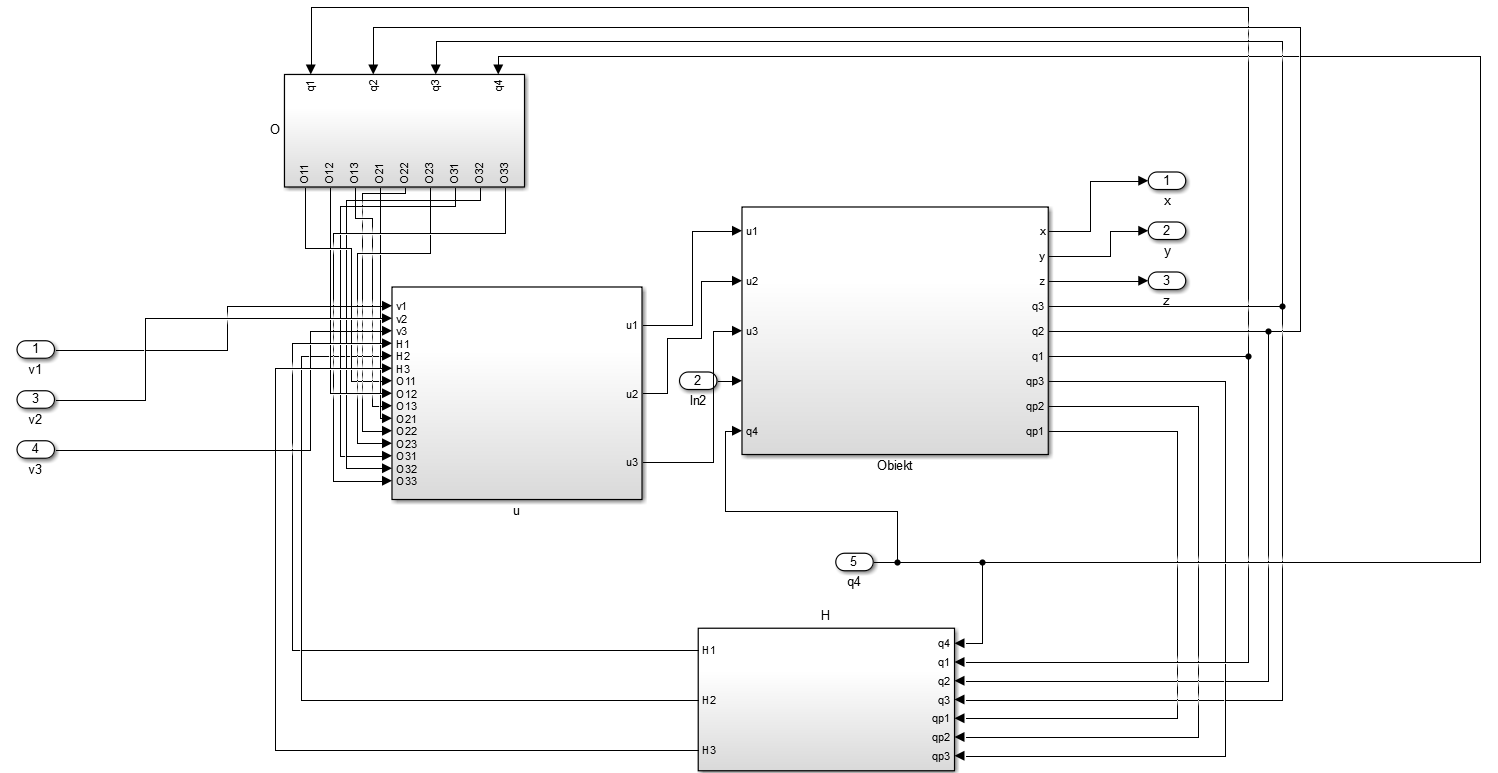
\includegraphics[width=1\textwidth]{08.png}
\caption{\label{fig:blok5}Podsystem Układ.}
\end{figure}


Pierwszym utworzonym blokiem był blok $H$ wynikający z równania 
\begin{equation}
H=P -JF(q)(C(q, \dot{q})\dot{q} + D(q))
\end{equation} 
Jego zawartość została podzielona na bloki $M, N, F, J, G, E, P$.
Bloki $M$ oraz $F$ są kopią bloków z podsystemu Dynamiki i mają za zadanie utworzyć $F(q)$, czyli odwrotność macierzy bezwładności $M(q)$. Blok $J$ odpowiedzialny jest za utworzenie macierzy Jacobiego $J(q)$. 
$$
J(q)=\left[
      \begin{array}{ccc}
         J_{11} & J_{12} & J_{13}\\ 
         J_{21} &J_{22} & J_{23}\\
         J_{31} & J_{32} & J_{33}
         \end{array}
      \right]
      $$
Pozostałe bloki $E, G, P, N$ wynikają bezpośrednio z obliczeń macierzy równania $H$. W pierwszej kolejności przeanalizowano kwestię bloku $P$. Niech
\begin{equation}
P_i=\dot{q}^T\frac{∂^2k_i}{∂q^2}\dot{q}, \ \ i=1,...,p.
\end{equation}
Z mnożenia macierzy można dojść do wniosku, że jest to skalar zależny od wartości $q_i$ oraz $\dot{q_i}$, według wzoru
\begin{eqnarray}
P_i=\left[
      \begin{array}{ccc}
         \dot{q_{1}} &\dot{q_{2}} & \dot{q_{3}}\\ 
         \end{array}
      \right]\left[
      \begin{array}{ccc}
         P_{i11} &P_{i12} & P_{i13}\\ 
         P_{i21} &P_{i22} & P_{i23}\\ 
         P_{i31} &P_{i32} & P_{i33}
         \end{array}
      \right]\left[
      \begin{array}{c}
         \dot{q}_1 \\
         \dot{q}_2 \\
         \dot{q}_3
         \end{array}
      \right], \ \ i=1,...,p.
\end{eqnarray}

      
gdzie:
\begin{eqnarray}
P_{111}&=&-c_1(a_2c_2+a_3c_3+d_6s_4),\\ \nonumber
P_{112}&=&-\sin(q_1)(-a_2\sin{q_2}+a_3\cos{q_3}+d_6\sin{q_4}),\\ \nonumber
P_{113}&=&-s_1(a_2c_2-a_3s_3+d_6s_4),\\ \nonumber
P_{121}&=&a_2s_1s_2,\\ \nonumber
P_{122}&=&-a_2c_1c_2,\\ \nonumber
P_{132}&=&0,\\ \nonumber
P_{131}&=&a_3s_1s_3,\\ \nonumber
P_{132}&=&0,\\ \nonumber
P_{133}&=&-a_3c_1c_3,\\ \nonumber
P_{211}&=&0,\\ \nonumber
P_{212}&=&0,\\ \nonumber
P_{213}&=&0,\\ \nonumber
P_{221}&=&0,\\ \nonumber
P_{222}&=&a_2s_2,\\ \nonumber
P_{223}&=&0,\\ \nonumber
P_{231}&=&0,\\ \nonumber
P_{232}&=&0,\\ \nonumber
P_{233}&=&a_3s_3,\\ \nonumber
P_{311}&=&-s_1(a_2c_2+a_3c_3+d_6s_4),\\ \nonumber
P_{312}&=&-a_2c_1s_2,\\ \nonumber
P_{313}&=&-a_3c_1s_3,\\ \nonumber
P_{321}&=&-a_2c_1s_2,\\ \nonumber
P_{322}&=&-a_2s_1c_2,\\ \nonumber
P_{323}&=&0,\\ \nonumber
P_{331}&=&-a_3c_1s_3,\\ \nonumber
P_{332}&=&0,\\ \nonumber
P_{333}&=&-a_3s_1c_3.
\end{eqnarray}
Po wymnożeniu uzyskano
\begin{eqnarray}
P_1&=&\dot{q}_1(-\dot{q}_1c_1(a_2c_2+a_3c_3+d_6s_4)+\dot{q}_2a_2s_1s_2-\dot{q}_3a_3s_1s_3)\\ \nonumber
&+&\dot{q}_2(-\dot{q}_1s_1(-a_2s_2+a_3c_3+d_6s_4)-\dot{q}_2a_2c_1c_2)\\ \nonumber
&+&\dot{q}_3(-\dot{q}_1s_1(a_2c_2-a_3s_3+d_6s_4)-\dot{q}_3c_1c_3),\\  \nonumber
P_2&=&\dot{q}_2(\dot{q}_2a_2s_2)+\dot{q}_3\dot{q}_3a_3s_3,\\  \nonumber
P_3&=&\dot{q}_1(-\dot{q}_1s_1(a_2c_2+a_3c_3+d_6s_4)-\dot{q}_2a_2c_1s_2-\dot{q}_3a_3c_1s_3)\\ \nonumber
&+&\dot{q}_2(-\dot{q}_1a_2c_1s_2-\dot{q}_2a_2s_1c_2)+\dot{q}_3(-\dot{q}_1a_3c_1s_3-\dot{q}_3a_3s_1c_3).
\end{eqnarray}

Blok G wynika z mnożenia $J(q)F(q)=G(q)$. W celu utworzenia macierzy $G(q)$ wykorzystano składowe macierzy Jacobiego oraz odwrotności macierzy bezwładności. Macierz ta ma postać
$$
G(q)=\left[
      \begin{array}{ccc}
         G_{11} & G_{12} & G_{13}\\ 
         G_{21} &G_{22} & G_{23}\\
         G_{31} & G_{32} & G_{33}
         \end{array}
      \right]
      $$
gdzie
\begin{eqnarray}
G_{11}&=&J_{11}F_{11},\\ \nonumber
G_{12}&=&J_{12}F_{22}+J_{13}F_{23},\\ \nonumber
G_{13}&=&J_{12}F_{22}+J_{13}F_{33},\\ \nonumber
G_{21}&=&0,\\ \nonumber
G_{22}&=&J_{22}F_{22}+J_{23}F_{23},\\ \nonumber
G_{23}&=&J_{22}F_{23}+J_{23}F_{33},\\ \nonumber
G_{31}&=&J_{32}F_{11},\\ \nonumber
G_{32}&=&J_{32}F_{22}+J_{33}F_{23},\\ \nonumber
G_{33}&=&J_{32}F_{23}+J_{33}F_{33}.
\end{eqnarray}


W równaniu dokonywane jest działanie na macierzach $C(q, \dot{q})\dot{q} + D(q)$ dające wektor, który oznaczono jako $E(q,\dot{q})$. Za niego odpowiedzialny jest właśnie blok $E$. Jego składowe to
$$
E(q, \dot{q})=\left[
      \begin{array}{ccc}
         C_{11} & C_{12} & C_{13}\\ 
         -C_{12} &0 & C_{23}\\
         -C_{13} & C_{32} & 0
         \end{array}
      \right]\left[
      \begin{array}{c}
      \dot{q_{1}} \\
         \dot{q_{2}} \\
         \dot{q_{3}}
         \end{array}
      \right]+\left[
      \begin{array}{c}
      D_1 \\
         D_2 \\
         D_3
         \end{array}
      \right] =    \left[
      \begin{array}{c}
      C_{11}\dot{q}_1+C_{12}\dot{q}_2+C_{13}\dot{q}_3+D_1 \\
        -C_{12}\dot{q}_1+C_{23}\dot{q}_3+D_2\\
         -C_{13}\dot{q}_1+C_{32}\dot{q}_2+D_3
         \end{array}
      \right].
      $$
Do zaimplementowania bloku $E$ wykorzystano wcześniej utworzone bloki $C$ oraz $D$. Ostatni Blok $N$ zaś jest wynikiem mnożenia $G(q)E(q,\dot{q})=N(q, \dot{q})$.
\begin{eqnarray}
N(q, \dot{q})=\left[
      \begin{array}{c}
      G_{11}E_1+G_{12}E_2+G_{13}E_3 \\
     G_{21}E_1+G_{22}E_2+G_{23}E_3 \\
          G_{31}E_1+G_{32}E_2+G_{33}E_3 \\
         \end{array}
      \right].
\end{eqnarray}


Ostatecznie, by uzyskać składowe wektora $H(q)$ należy na końcu odjąć wektor $N(q, \dot{q})$ od $P$. 


Drugim blokiem w podsystemie Układ jest blok $O$, wyliczający macierz $O(q)$, która jest odwrotnością wcześniej wyliczonej macierzy $G(q)$. Sposób wyliczenia jest standardowy, wykorzystujący odwrotność wyznacznika tej macierzy. Wyznacznik macierzy $G(q)$ równa się
\begin{equation}
det(G(q))=G_{11}G_{22}G_{33}+G_{31}G_{12}G_{23}-G_{11}G_{32}G_{23}-G_{31}G_{22}G_{13}
\end{equation}
Uzyskano macierz
$$
O(q)=G^{-1}(q)=\left[
      \begin{array}{ccc}
         O_{11} & O_{12} & O_{13}\\ 
         O_{21} &O_{22} & O_{23}\\
         O_{31} & O_{32} & O_{33}
         \end{array}
      \right],
      $$
      z elementami równymi odpowiednio
      \begin{eqnarray}
      O_{11}&=&\frac{1}{det(G(q))}(G_{22}G_{33}-G_{23}G_{32}),\\ \nonumber
      O_{12}&=&\frac{1}{det(G(q))}(G_{13}G_{32}-G_{11}G_{33}),\\ \nonumber
      O_{13}&=&\frac{1}{det(G(q))}(G_{12}G_{23}-G_{13}G_{22}),\\ \nonumber
      O_{21}&=&\frac{1}{det(G(q))}(G_{23}G_{31}),\\ \nonumber
      O_{22}&=&\frac{1}{det(G(q))}(G_{11}G_{33}-G_{13}G_{31}),\\ \nonumber
      O_{23}&=&\frac{1}{det(G(q))}(-G_{11}G_{23}),\\ \nonumber
      O_{31}&=&\frac{1}{det(G(q))}(-G_{22}G_{31}),\\ \nonumber
      O_{32}&=&\frac{1}{det(G(q))}(G_{12}G_{31}-G_{11}G_{32}),\\ \nonumber
      O_{33}&=&\frac{1}{det(G(q))}(G_{11}G_{22}).
      \end{eqnarray}
 
Ostatnim blokiem w Układzie jest blok $U$ odpowiedzialny za połączenie wyników z bloków $H$ oraz $O$ ze sprzężenia zwrotnego. Jego działanie jest zależne od równania
$$
u=\left[
\begin{array}{ccc}
O_{11} & O_{12} & O_{13}\\ 
         O_{21} &O_{22} & O_{23}\\
         O_{31} & O_{32} & O_{33}
         \end{array}
      \right]\left[
      \begin{array}{c}
      v_1-H_1\\
      v_2-H_2\\
      v_3-H_3\\
      \end{array}
      \right]=\left[
      \begin{array}{c}
      O_{11}(v_1-H_1)+O_{12}(v_2-H_2)+O_{13}(v_3-H_3)\\
      O_{21}(v_1-H_1)+O_{22}(v_2-H_2)+O_{23}(v_3-H_3)\\
      O_{31}(v_1-H_1)+O_{32}(v_2-H_2)+O_{33}(v_3-H_3)
      \end{array}
            \right].
$$



\chapter{Sterowanie układem odsprzężonym}
\section{Generator trajektorii zadanej}
W celu przeprowadzenia analizy jakości opracowanego algorytmu, trzeba określić jaka trajektoria ruchu manipulatora będzie realizowana. Z tego powodu utworzono dodatkowy blok nazwany Generatorem, który będzie generował żądane współrzędne chwytaka. Na początek wybrano ruch śrubowy o następujących wzorach:
\begin{eqnarray}\label{row4.1}
\left\{ \begin{array}{lll}
x_d(t)&=& 0.05\cos\left(t\right)\\
y_d(t)&=&0.05\sin\left(t\right)\\
z_d(t)&=&\frac{t}{100} \\
\end{array} \right.
\end{eqnarray}


Tak jak w poprzednich rozdziałach, uwzględniono, że idealne różniczkowanie numeryczne nie istnieje. Zamiast tego zamodelowano najwyższe pochodne, a następnie scałkowano je z odpowiednimi warunkami początkowymi
\begin{eqnarray}
x_d(t)&=& 0.05\cos\left(t\right),\\ \nonumber
\dot{x}_d(t)&=& -0.05\sin\left(t\right),\\ \nonumber
\ddot{x}_d(t)&=& -0.05\cos\left(t\right),\\ \nonumber
x_d(0)&=&0.05,\\ \nonumber
\dot{x}_d(0)&=&0,\\ \nonumber
y_d(t)&=& 0.05\sin\left(t\right),\\ \nonumber
\dot{y}_d(t)&=&0.05\cos\left(t\right),\\ \nonumber
\ddot{y}_d(t)&=& -0.05\sin\left(t\right),\\ \nonumber
y_d(0)&=&0,\\ \nonumber
\dot{y}_d(0)&=&0.05,\\ \nonumber
\end{eqnarray}
\begin{eqnarray}
z_d(t)&=& \frac{t}{100},\\ \nonumber
\dot{z}_d(t)&=& \frac{1}{100},\\ \nonumber
\ddot{z}_d(t)&=& 0,\\ \nonumber
z_d(t)&=&0,\\ \nonumber
\dot{z}_d(t)&=&\frac{1}{100}.
\end{eqnarray}

Z tak zaimplementowanym Generatorem będzie określana dla sygnału wejściowego odpowiednia trajektoria ruchu chwytaka. Ta z kolei będzie na bieżąco sprawdzana z rzeczywistymi współrzędnymi efektora IRb-6, co pozwoli na wyliczenie uchybu układu.
\section{Regulacja PD z korekcją}
 Posiadając generator trajektorii, można przystąpić do tworzenia algorytmu gwarantującego zbieżność błędu śledzenia. Zaimplementowany zostanie regulator PD określony zależnością
 \begin{eqnarray}
 \label{row4.4}
 v&=& \ddot{y}_{CHd}-K_d\dot{e}_y-K_pe_y,
 \end{eqnarray}
 gdzie
  \begin{eqnarray}\label{row4.5}
 e_y&=&y_{CH}-y_{CHd}.
 \end{eqnarray}
Regulator ten został opisany w \cite{b1}.  Stałe $K_d$ oraz $K_p$ są nastawami regulatora. Wartość $e_y$ oraz jej pochodna są sygnałami uchybu wynikającego z różnicy pomiędzy rzeczywistym położeniem efektora w przestrzeni roboczej, a żądaną trajektorią określoną przez generator. 

Na podstawie wzoru (\ref{row4.4}) opisano zależność sygnału sterującego od uchybu
\begin{eqnarray}
v_1 &=& \ddot{x}_{d}-K_d(\dot{x}-\dot{x}_d)-K_p(x-x_d), \\ \nonumber
v_2 &=& \ddot{y}_{d}-K_d(\dot{y}-\dot{y}_d)-K_p(y-y_d), \\ \nonumber
v_3 &=& \ddot{z}_{d}-K_d(\dot{z}-\dot{z}_d)-K_p(z-z_d). \\ \nonumber
\end{eqnarray}
gdzie współrzędne $x_d$, $y_d$, $z_d$ oraz ich pochodne pochodzą z generatora trajektorii, a współrzędne $x$, $y$, $z$ można wyliczyć z kinematyki obiektu (\ref{row2.30}). 
Stałe współczynniki $K_p$ oraz $K_d$ dobrano uwzględniając zależność $K_p=10K_d$. Wypróbowano kilka rzędów wielkości wartości stałych, jednak symulacje przeprowadzono dla wartości 
\begin{itemize}
\item $K_p=100$,
\item $K_d=10$.
\end{itemize}
\newpage


W \cite{b1} wykorzystywano wartości stałych dziesięć razy mniejsze. Zwiększenie wartości stałych zmniejszy uchyb sterowania układu. Jednak będzie to też wymagało większej mocy obliczeniowej.
Cały schemat regulacji został przedstawiony na rysunku \ref{fig:blok8}.
\begin{figure}[ht]
\centering
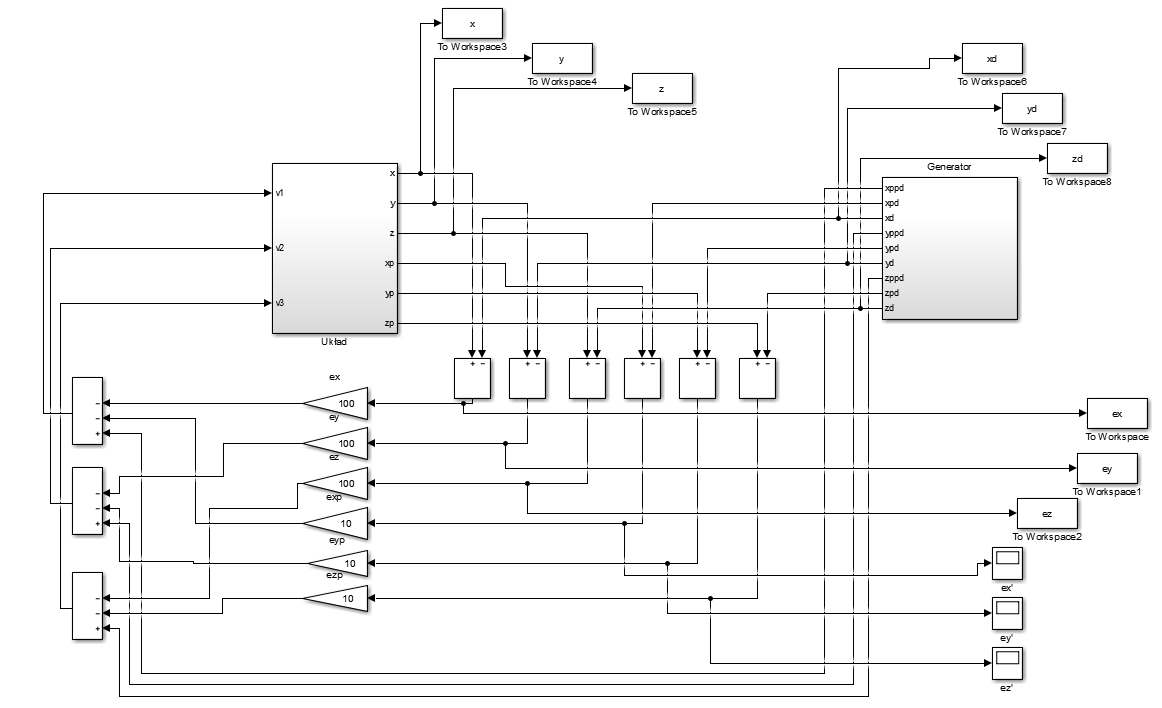
\includegraphics[width=1\textwidth]{13.png}
\caption{\label{fig:blok8}Regulacja PD z korekcją.}
\end{figure}
\chapter{Badania symulacyjne}
\section{Warunki symulacyjne}
W celu przetestowania skuteczności algorytmu odsprzęgania wejściowo-wyjściowego, dokonano symulacji sterowania manipulatorem IRb-6 dla konkretnych trajektorii efektora. Symulacje zostały przeprowadzone w programie Matlab i Simulink w wersji R2016b. Komputer, który przeprowadzał symulację miał następujące parametry:
\begin{itemize}
\item Procesor Intel(R) Core(TM) i7-8550U CPU 1.80 GHz,
\item Pamięć RAM 8.00 GB,
\item System 64-bitowy Windows 10.
\end{itemize}


Dla wszystkich symulacji wykorzystywano metodę całkowania ode23 o dokładności $10^{-10}$. 

Dla każdej trajektorii dobrano jednakowe warunki początkowe ustawienia manipulatora. Wynoszą one kolejno
\begin{eqnarray}
q_1(0)&=&1\approx 57.3^{\circ},\\ \nonumber
q_2(0)&=&0.4\approx 22.9^{\circ},\\ \nonumber
q_3(0)&=&0.1\approx 5.7^{\circ},\\ \nonumber
q_4(0)&=&1.6\approx 91.7^{\circ}. \nonumber
\end{eqnarray}

Konfiguracja początkowa została tak dobrana, by zminimalizować szansę osiągnięcia przez manipulator konfiguracji osobliwych, we wszystkich trajektoriach. Współrzędne efektora dla tej konfiguracji początkowej wynoszą
\begin{eqnarray}
x&=& 0.6354439932\approx 0.64, \\ \nonumber
y&=& -0.9449005978\approx -0.94,\\ \nonumber
z&=& 0.9104502922\approx 0.91. \nonumber
\end{eqnarray}

\newpage
\section{Ruch prostoliniowy}
Pierwszym testem dla sterowania będzie przemieszczanie efektora w przestrzeni roboczej po liniach prostych. Przeprowadzono pomiar 
\begin{itemize}
\item zależności położenia efektora w przestrzeni od czasu,
\item zależności uchybu położenia od czasu.
\item sygnały sterujące u(t)
\end{itemize}
Najpierw poprowadzono efektor wzdłuż osi $x$, po linii prostej. Ruch ten opisany jest zależnościami $x_d(t)=\frac{t}{10}$, $y_d=0$ oraz $z_d=0$.

Na rysunku \ref{odx} przedstawiono charakterystyki trajektorii zadanej oraz trajektorii rzeczywistej dla współrzędnej $x$.
Sygnały sterujące dla ruchu po linii prostej w kierunku osi OX zostały przedstawione na rysunku \ref{uodx}.
\hfill \break
\begin{figure}[!h]
\centering
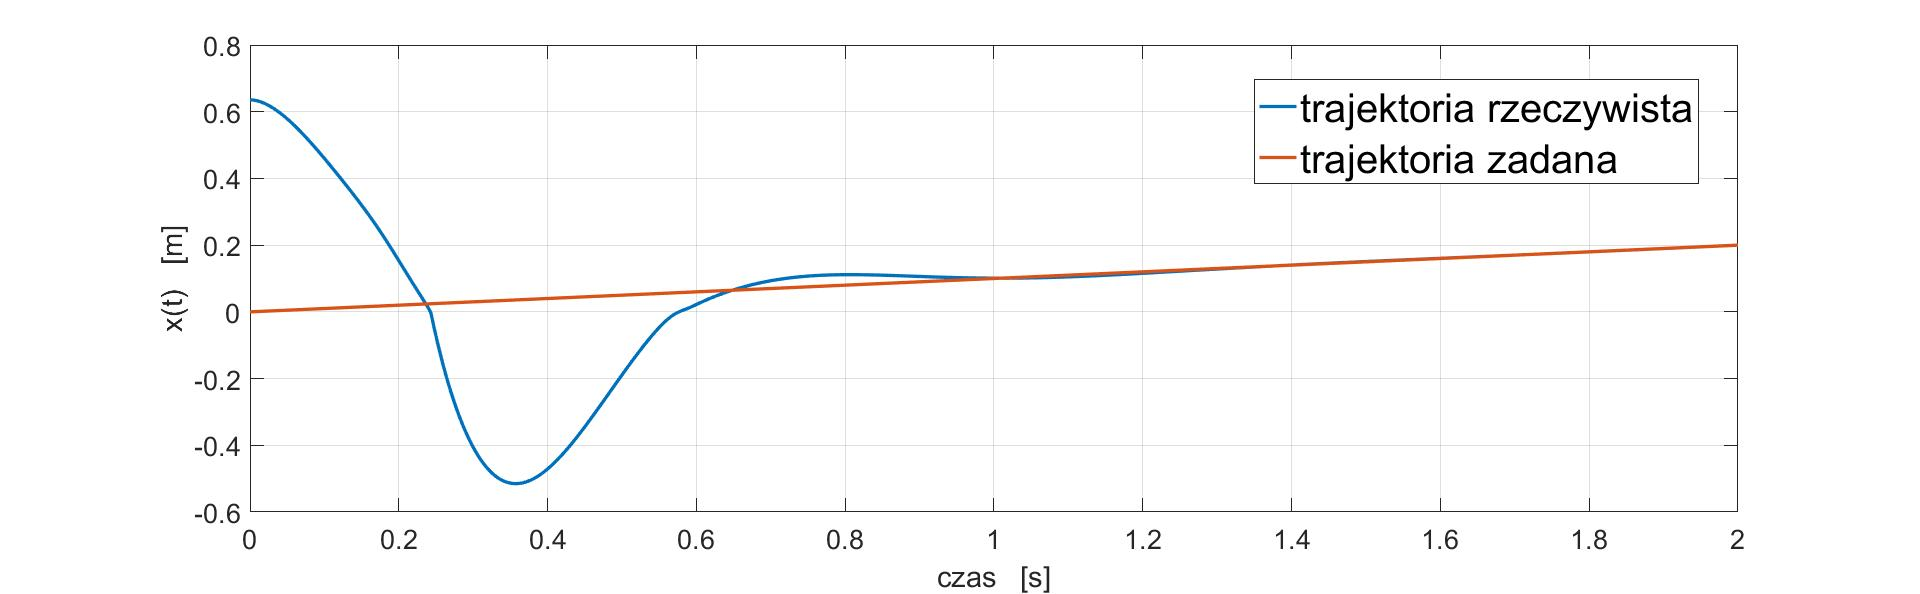
\includegraphics[width=1\textwidth]{odx.jpg}
\caption{\label{odx}Przebieg zmiennej $x(t)$ dla trajektorii zadanej oraz rzeczywistej.}
\end{figure}
\begin{figure}[!h]
\centering
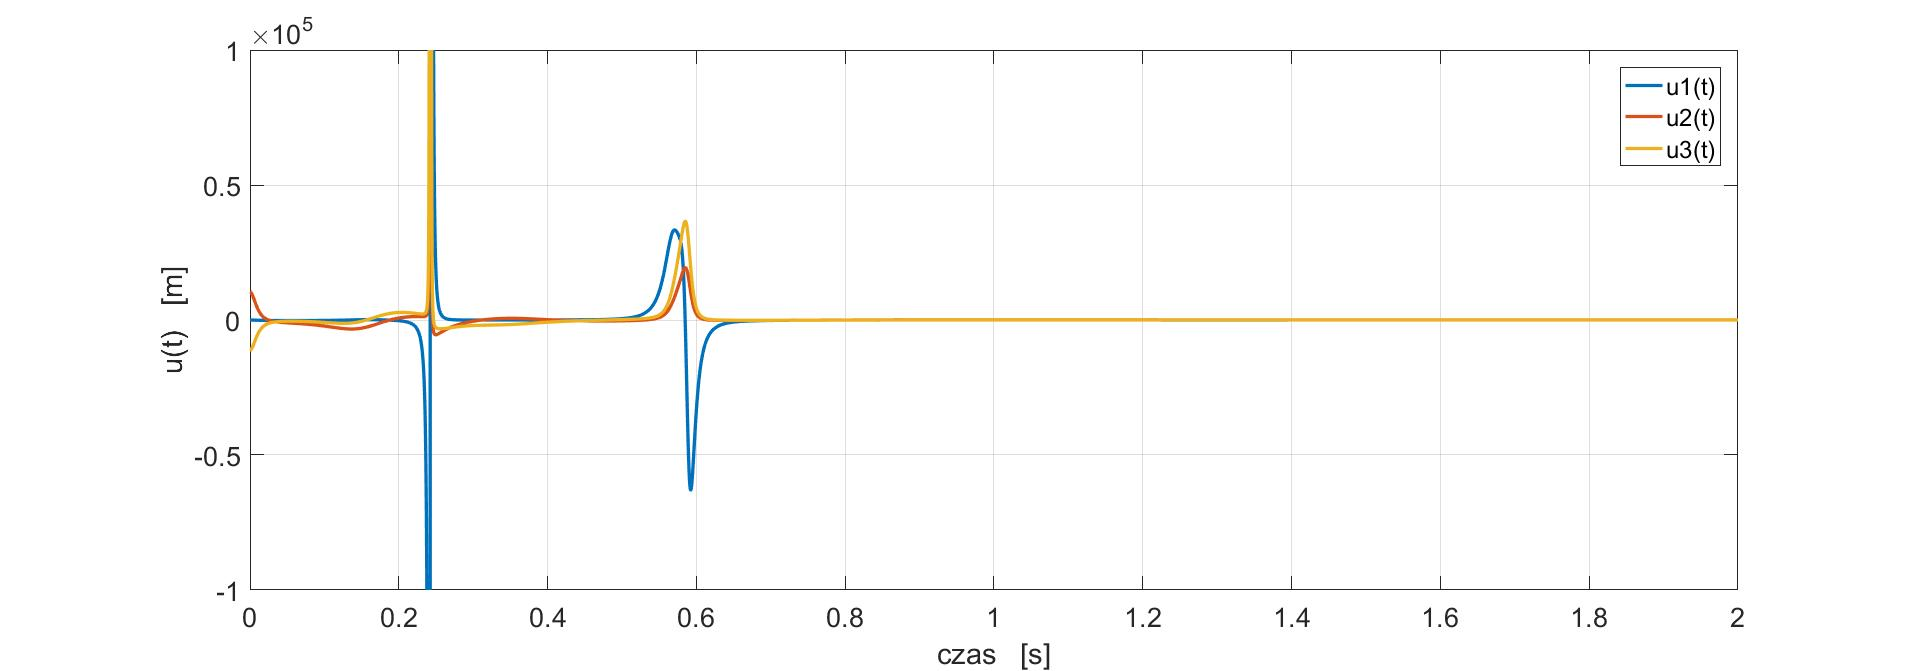
\includegraphics[width=1\textwidth]{uodx.jpg}
\caption{\label{uodx}Sygnały sterujące $u(t)$ dla ruchu po linii prostej w kierunku osi OX.}
\end{figure}
\newpage
Uchyb śledzenia linii prostej wzdłuż osi OX dla wszystkich współrzędnych maleje do zera, co można zaobserwować na wykresach \ref{exodx}, \ref{eyodx} oraz \ref{ezodx}.

\begin{figure}[!h]
\centering
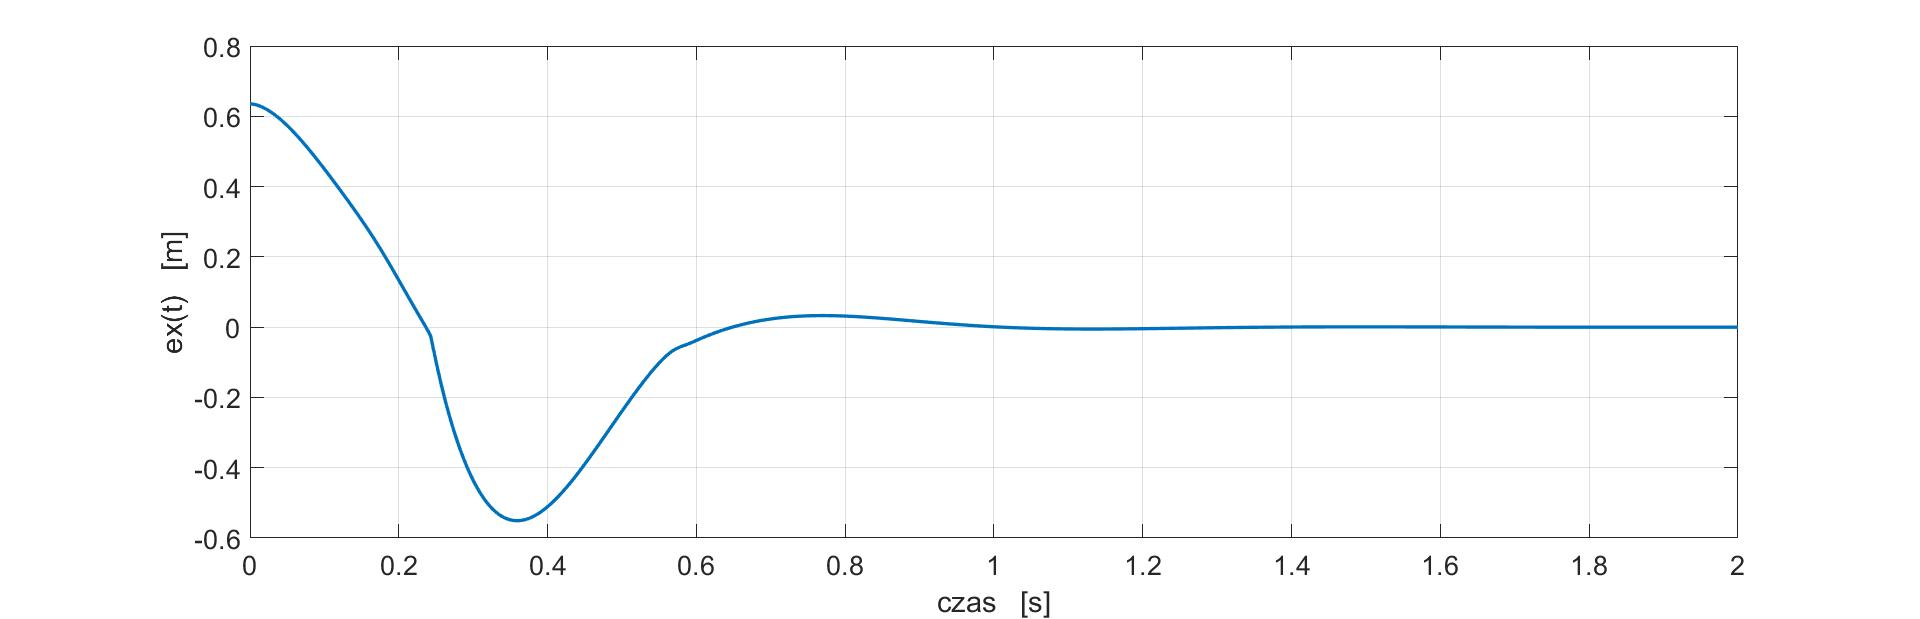
\includegraphics[width=1\textwidth]{exodx.jpg}
\caption{\label{exodx}Przebieg błędu $e_x(t)$ dla linii prostej wzdłuż osi OX.}
\end{figure}
\begin{figure}[!h]
\centering
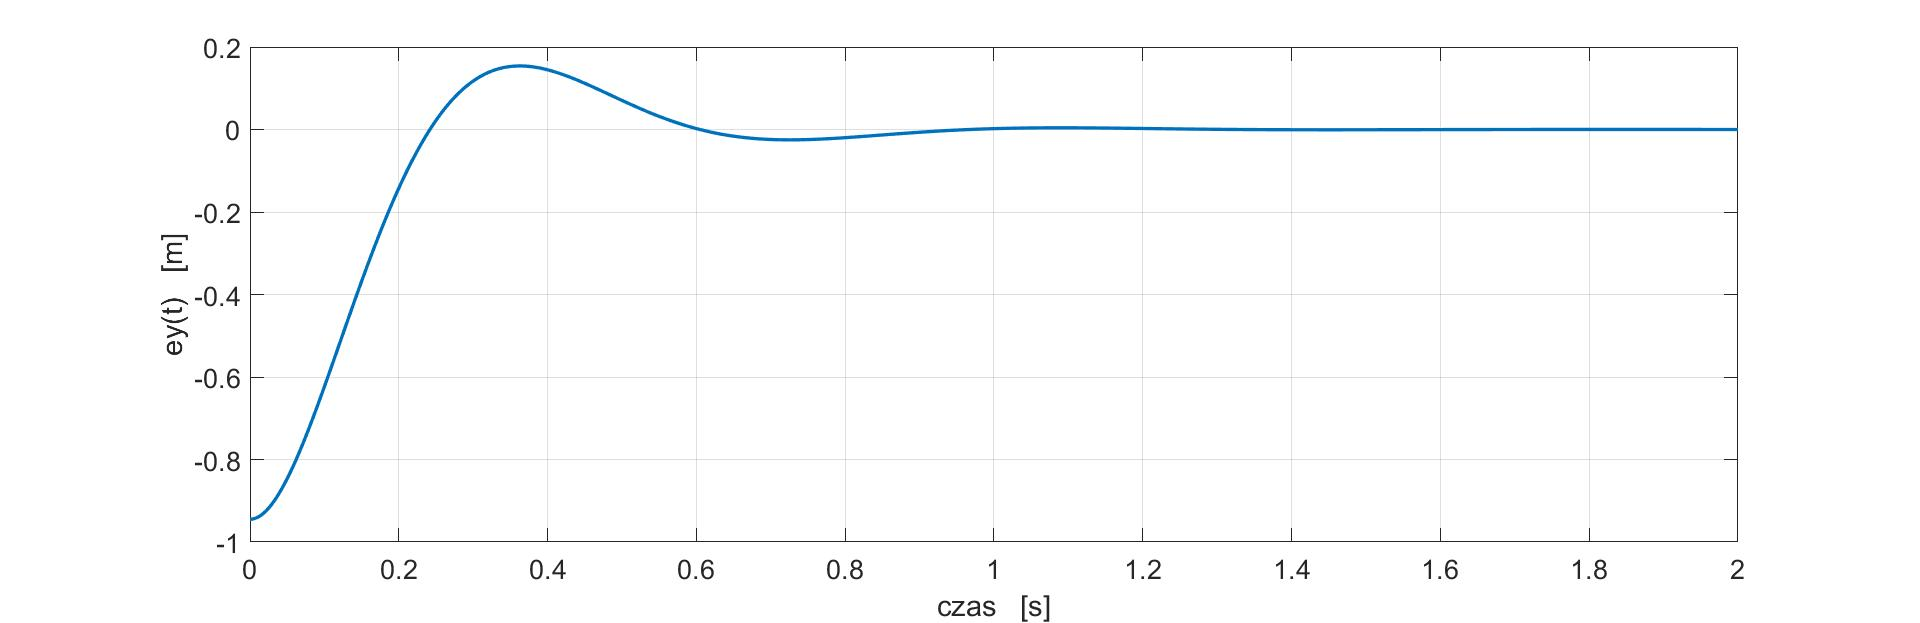
\includegraphics[width=1\textwidth]{eyodx.jpg}
\caption{\label{eyodx}Przebieg błędu $e_y(t)$ dla linii prostej wzdłuż osi OX.}
\end{figure}
\begin{figure}[!h]
\centering
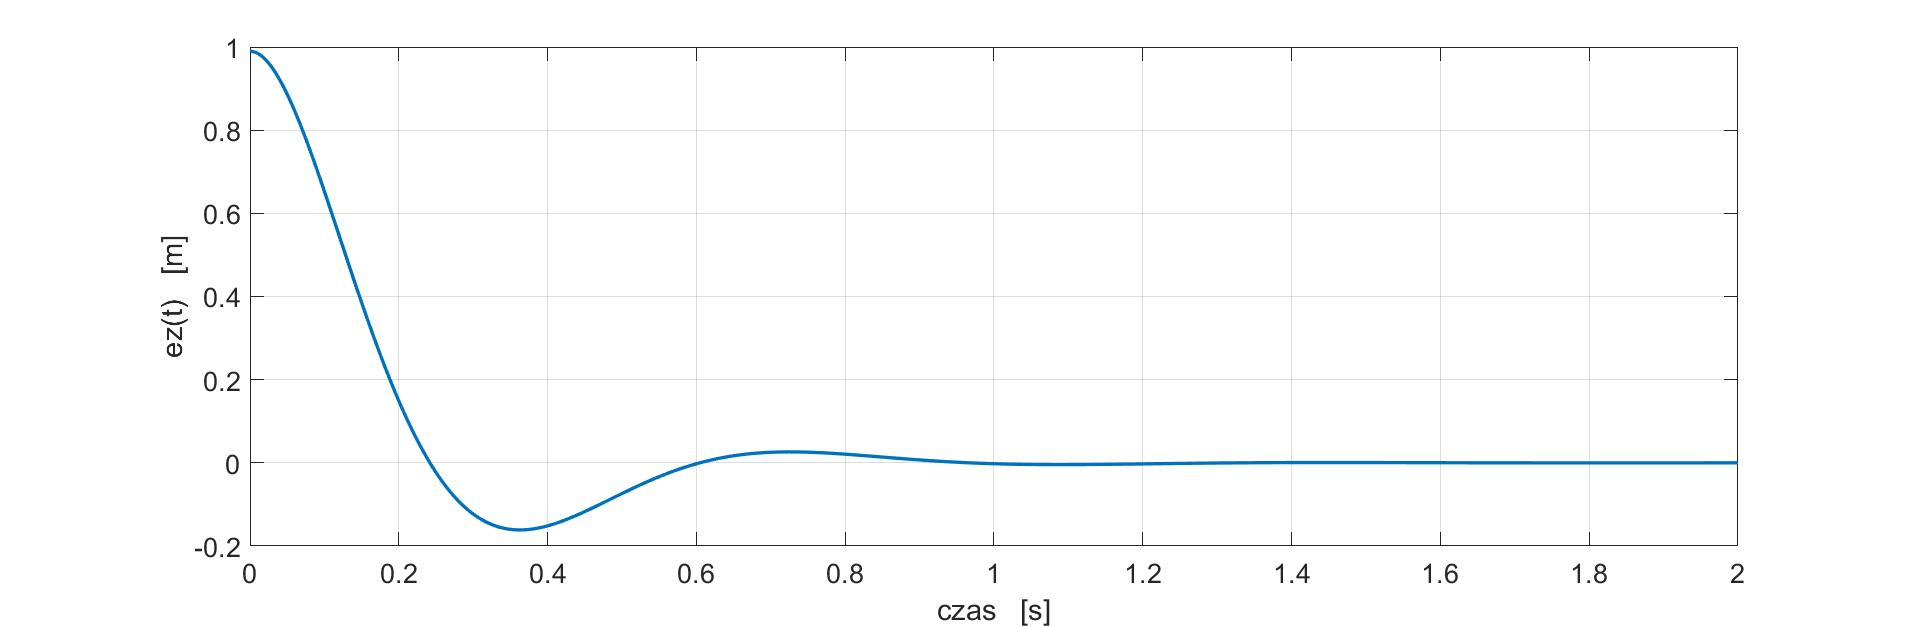
\includegraphics[width=1\textwidth]{ezodx.jpg}
\caption{\label{ezodx}Przebieg błędu $e_z(t)$ dla linii prostej wzdłuż osi OX.}
\end{figure}
\newpage
Na rysunku \ref{ody} przedstawiono charakterystykę $y(t)$ dla ruchu po linii prostej w kierunku osi OY. Ruch ten opisany jest zależnościami $x_d(t)=0$, $y_d=\frac{t}{10}$ oraz $z_d=0$. Tak samo jak w przypadku ruchu po linii prostej w kierunku osi OX wykreślono także zależności sygnałów sterujących od czasu na rysunku \ref{uody}.
\hfill \break
\begin{figure}[!h]
\centering
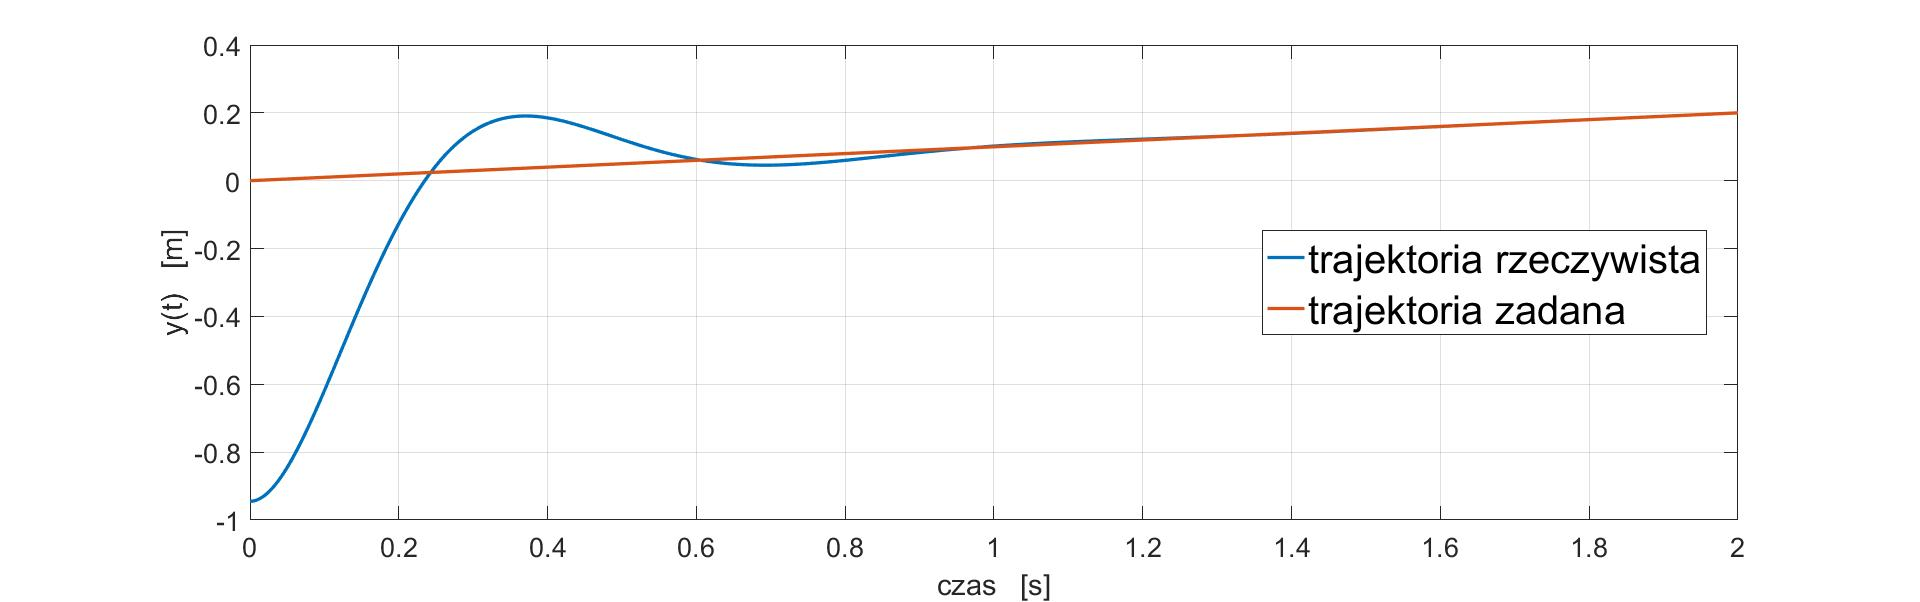
\includegraphics[width=1\textwidth]{ody.jpg}
\caption{\label{ody}Przebieg zmiennej $y(t)$ dla trajektorii zadanej oraz rzeczywistej.}
\end{figure}
\begin{figure}[!h]
\centering
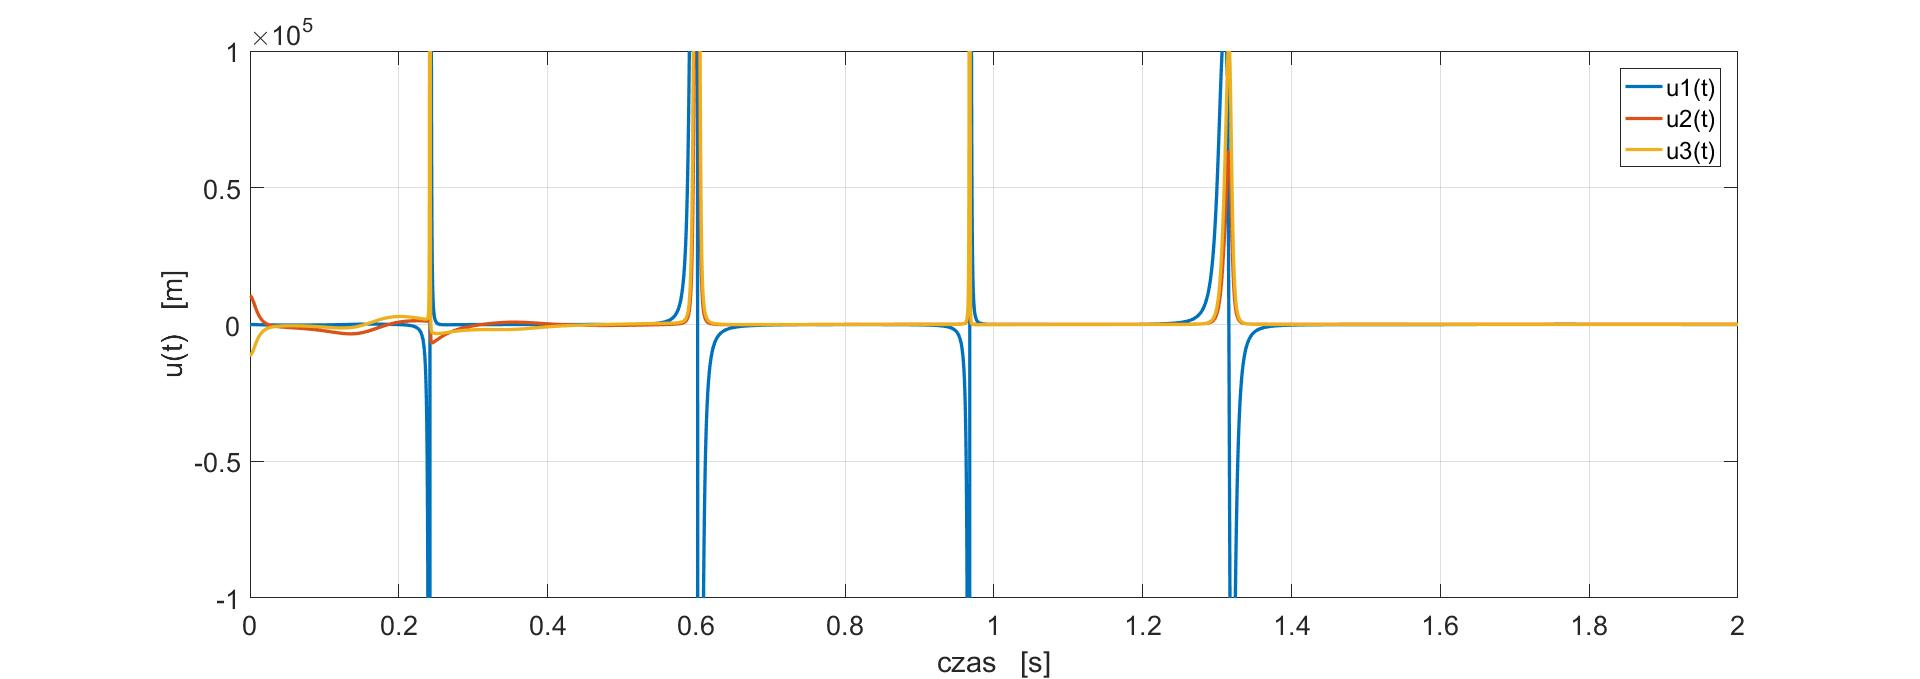
\includegraphics[width=1\textwidth]{uody.jpg}
\caption{\label{uody}Sygnały sterujące $u(t)$ dla ruchu po linii prostej w kierunku osi OY.}
\end{figure}
\newpage


Uchyb śledzenia linii prostej wzdłuż osi OY dla wszystkich współrzędnych maleje do zera, co można zaobserwować na wykresach \ref{exody}, \ref{eyody} oraz \ref{ezody}.

\begin{figure}[!h]
\centering
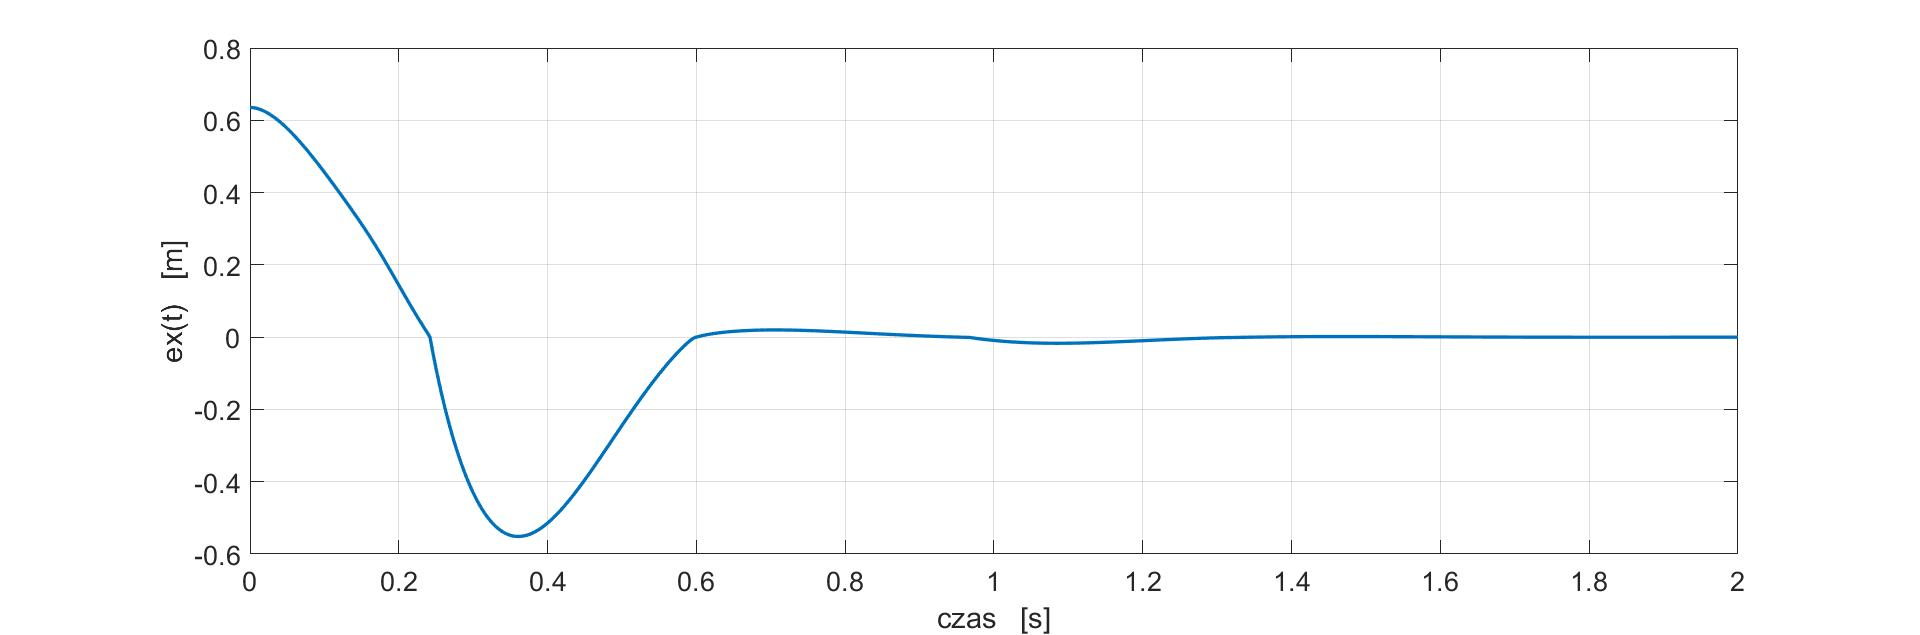
\includegraphics[width=1\textwidth]{exody.jpg}
\caption{\label{exody}Przebieg błędu $e_x(t)$ dla linii prostej wzdłuż osi OY.}
\end{figure}
\begin{figure}[!h]
\centering
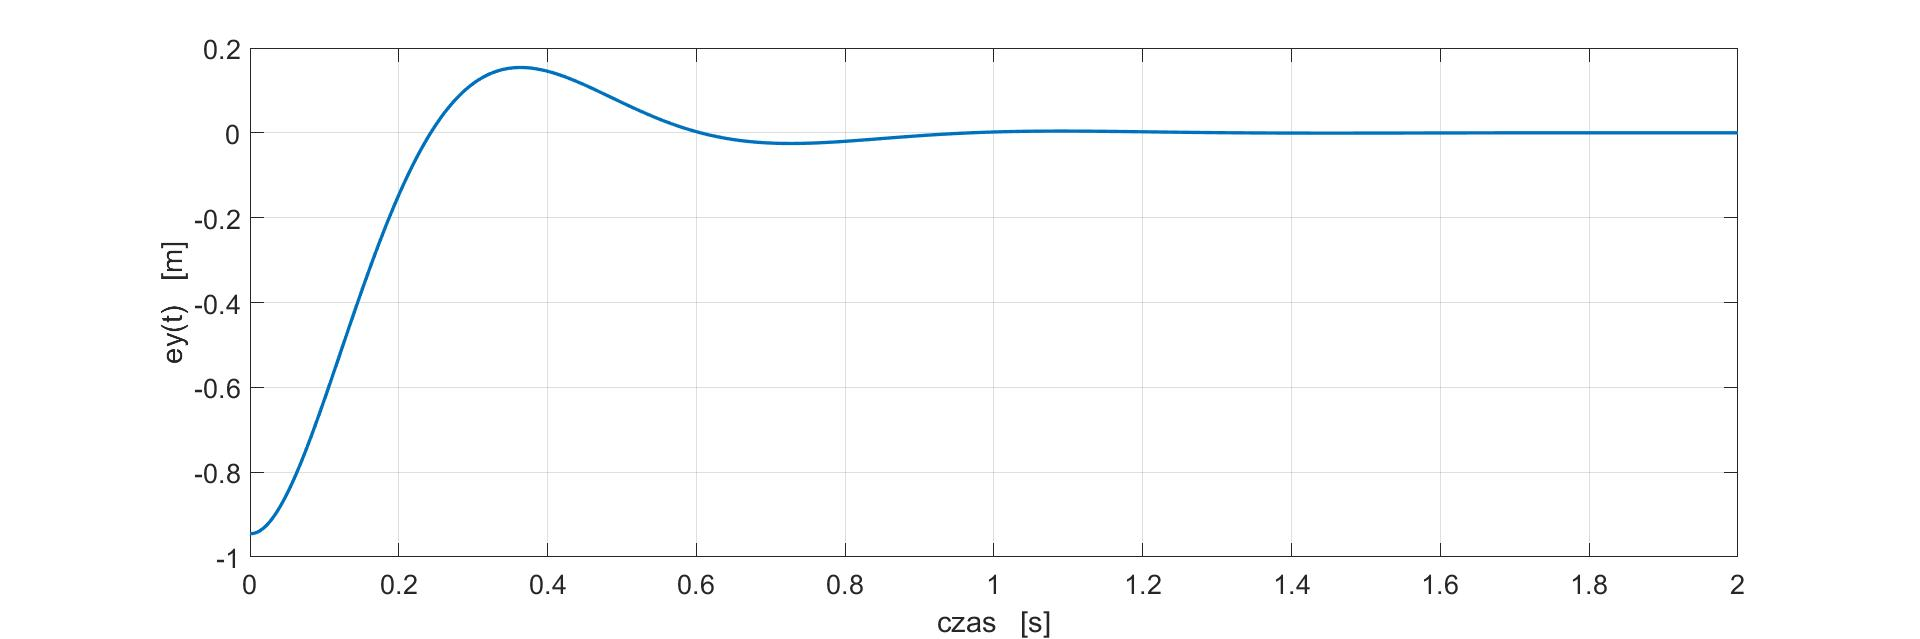
\includegraphics[width=1\textwidth]{eyody.jpg}
\caption{\label{eyody}Przebieg błędu $e_y(t)$ dla linii prostej wzdłuż osi OY.}
\end{figure}
\begin{figure}[!h]
\centering
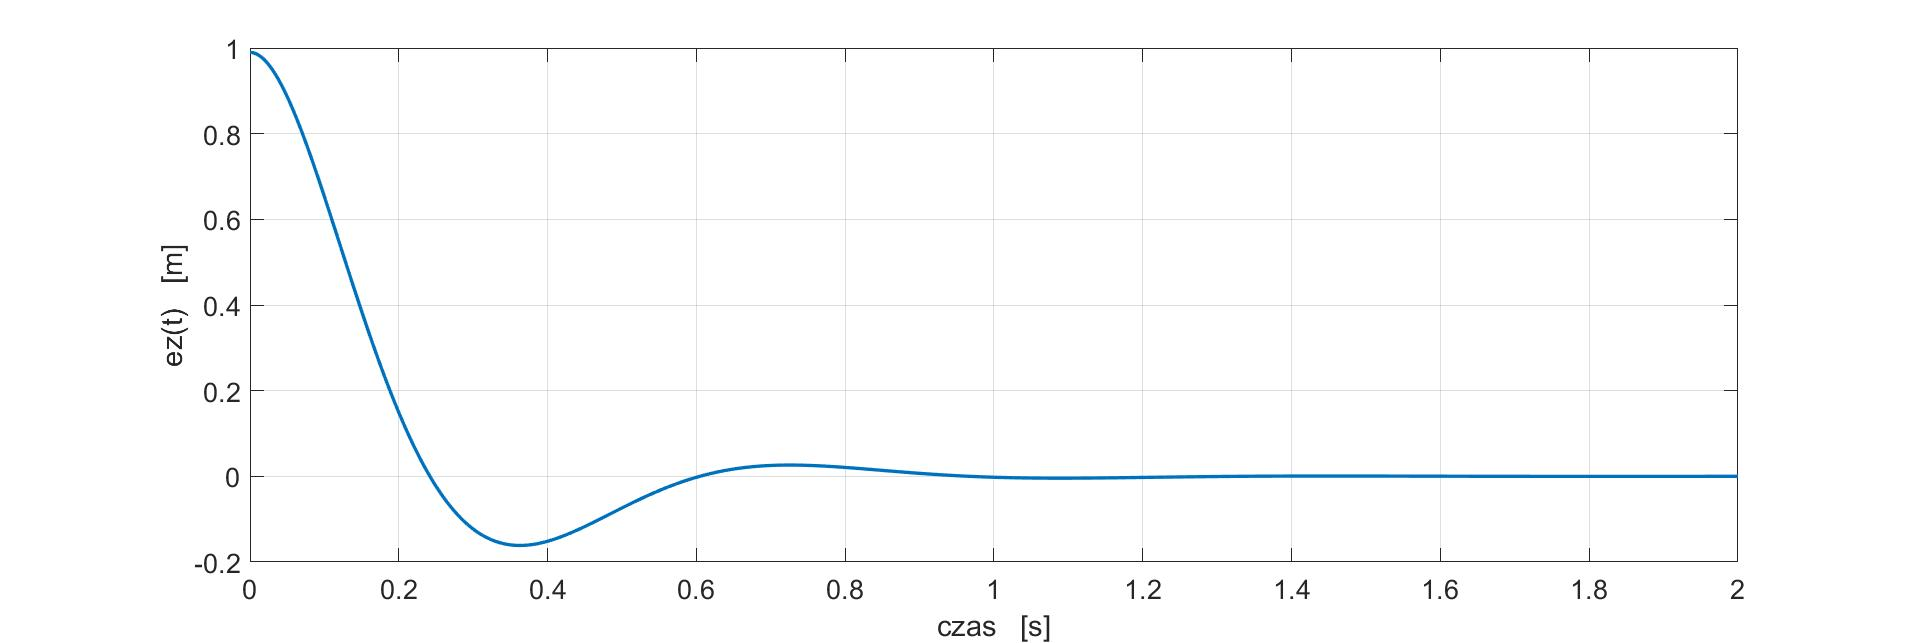
\includegraphics[width=1\textwidth]{ezody.jpg}
\caption{\label{ezody}Przebieg błędu $e_z(t)$ dla linii prostej wzdłuż osi OY.}
\end{figure}
\newpage
Na końcu poprowadzono efektor po linii prostej w kierunku osi OZ i sprawdzono charakterystyki trajektorii $z(t)$. Ruch ten opisany jest zależnościami $x_d(t)=0$, $y_d=0$ oraz $z_d=\frac{t}{10}$.
Trajektorię zadaną i rzeczywistą przedstawiono na rysunku \ref{odz}. Na rysunku \ref{uodz} zaprezentowano sygnały sterujące dla tego ruchu.
\hfill \break
\begin{figure}[!h]
\centering
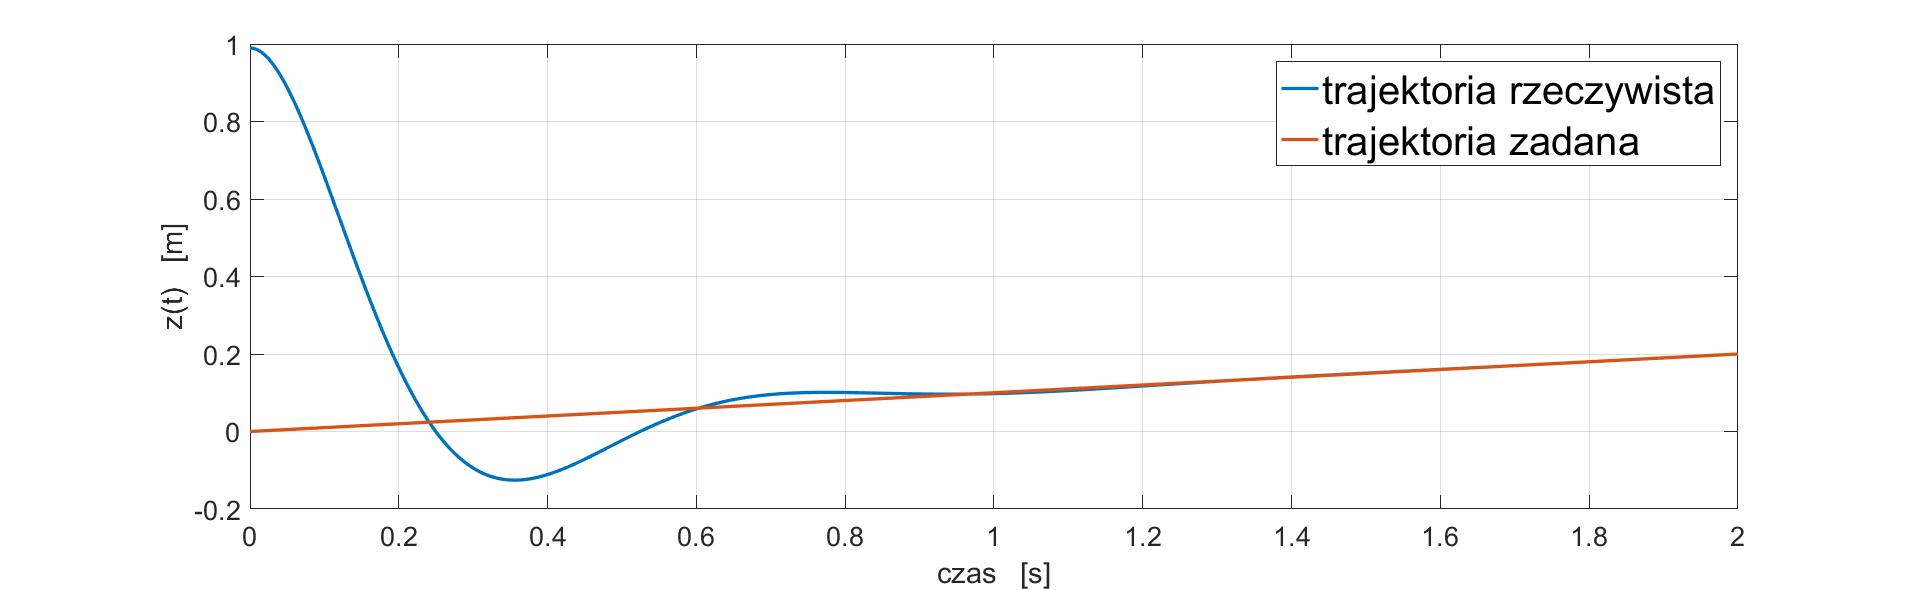
\includegraphics[width=1\textwidth]{odz.jpg}
\caption{\label{odz}Przebieg zmiennej $z(t)$ dla trajektorii zadanej oraz rzeczywistej.}
\end{figure}
\begin{figure}[!h]
\centering
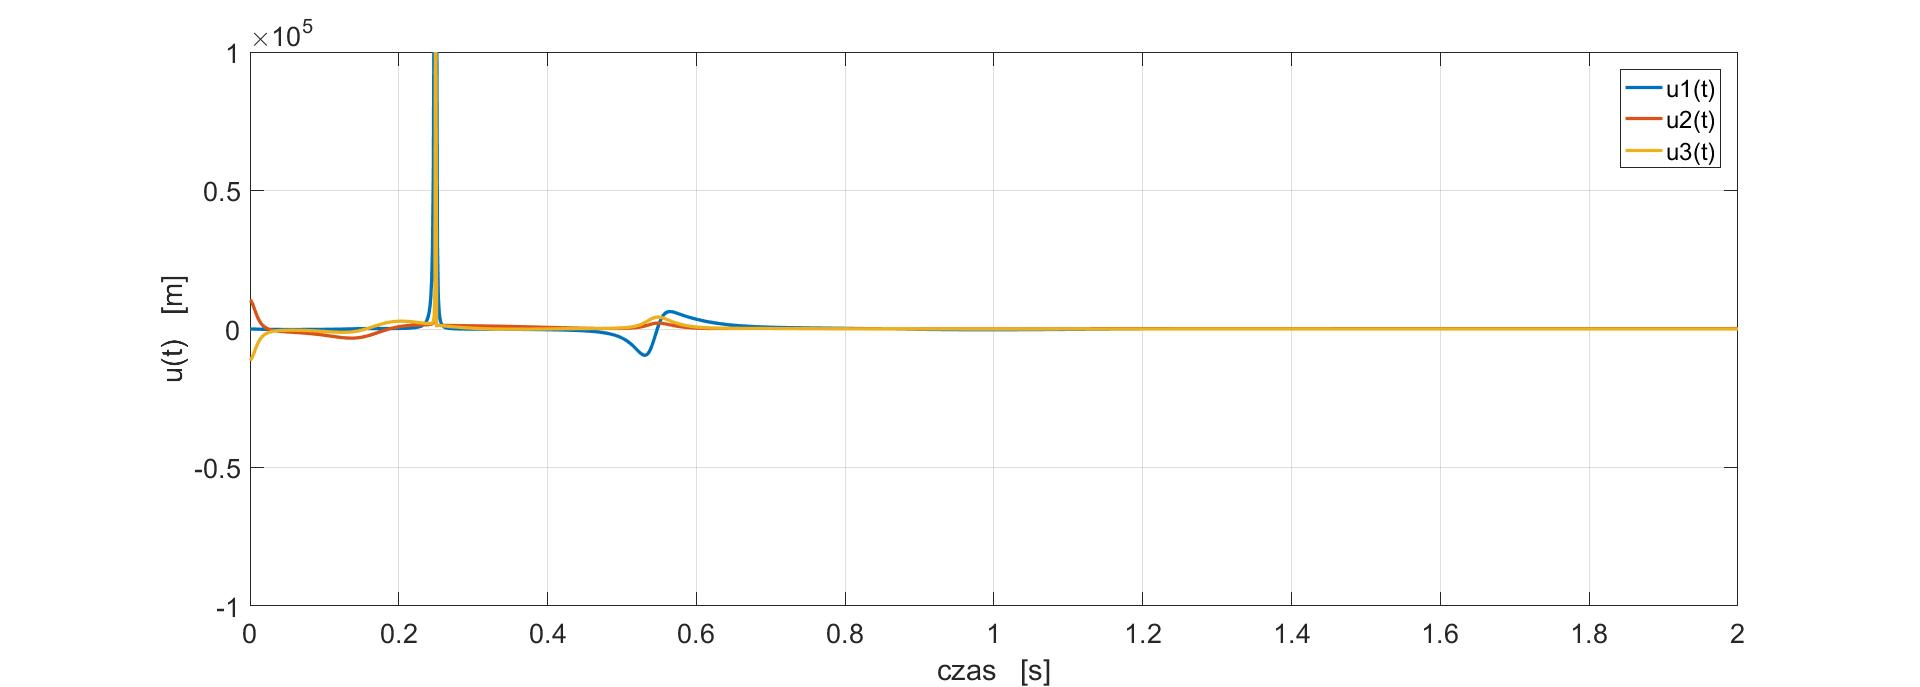
\includegraphics[width=1\textwidth]{uodz.jpg}
\caption{\label{uodz}Sygnały sterujące $u(t)$ dla ruchu po linii prostej w kierunku osi OZ.}
\end{figure}
\newpage
Uchyb śledzenia linii prostej wzdłuż osi OZ dla wszystkich współrzędnych maleje do zera, co można zaobserwować na wykresach \ref{exodz}, \ref{eyodz} oraz \ref{ezodz}.

\begin{figure}[!h]
\centering
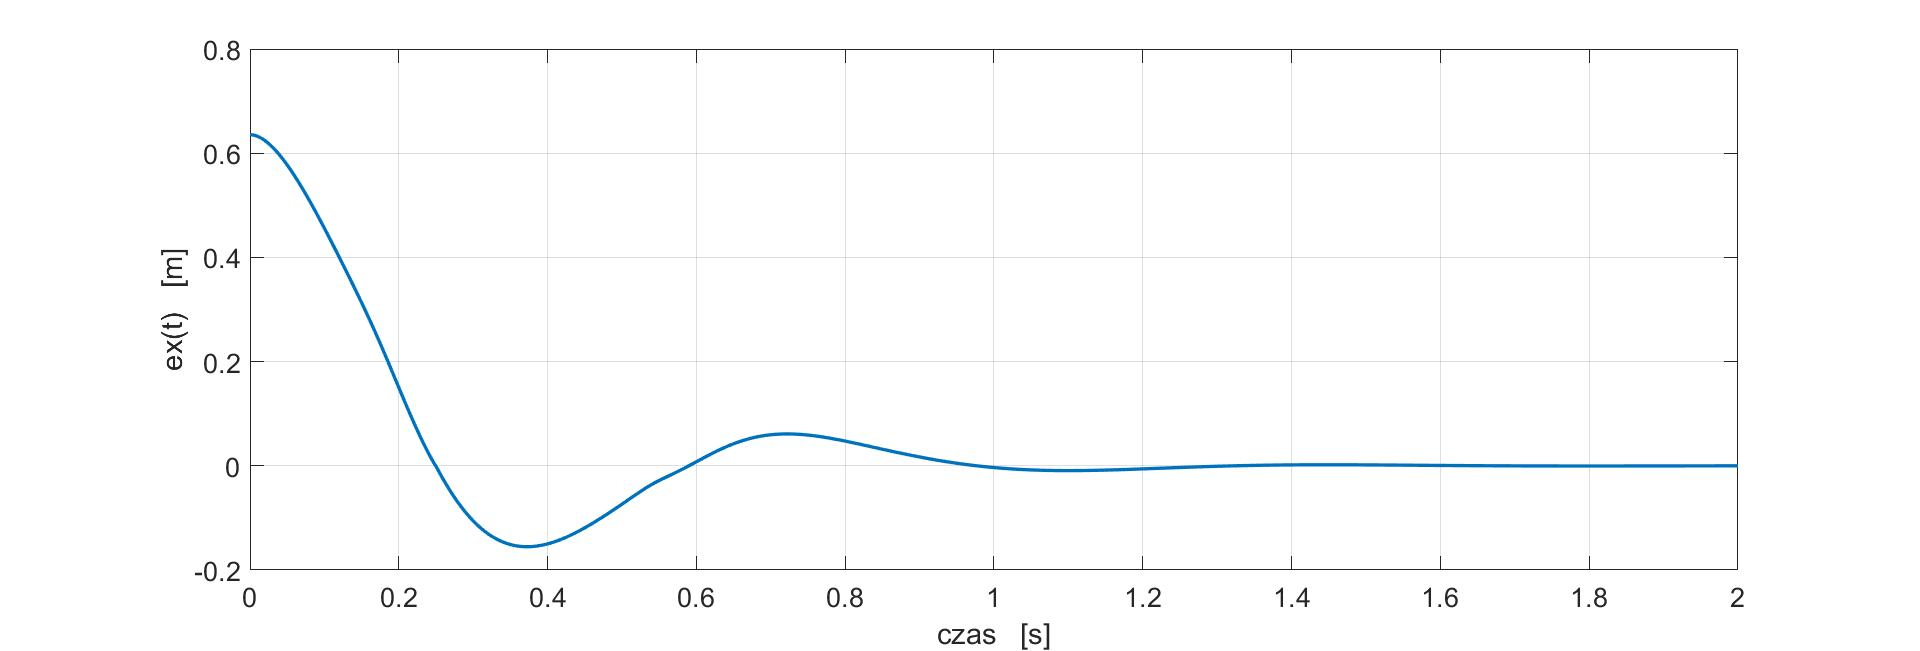
\includegraphics[width=1\textwidth]{exodz.jpg}
\caption{\label{exodz}Przebieg błędu $e_x(t)$ dla linii prostej wzdłuż osi OZ.}
\end{figure}
\begin{figure}[!h]
\centering
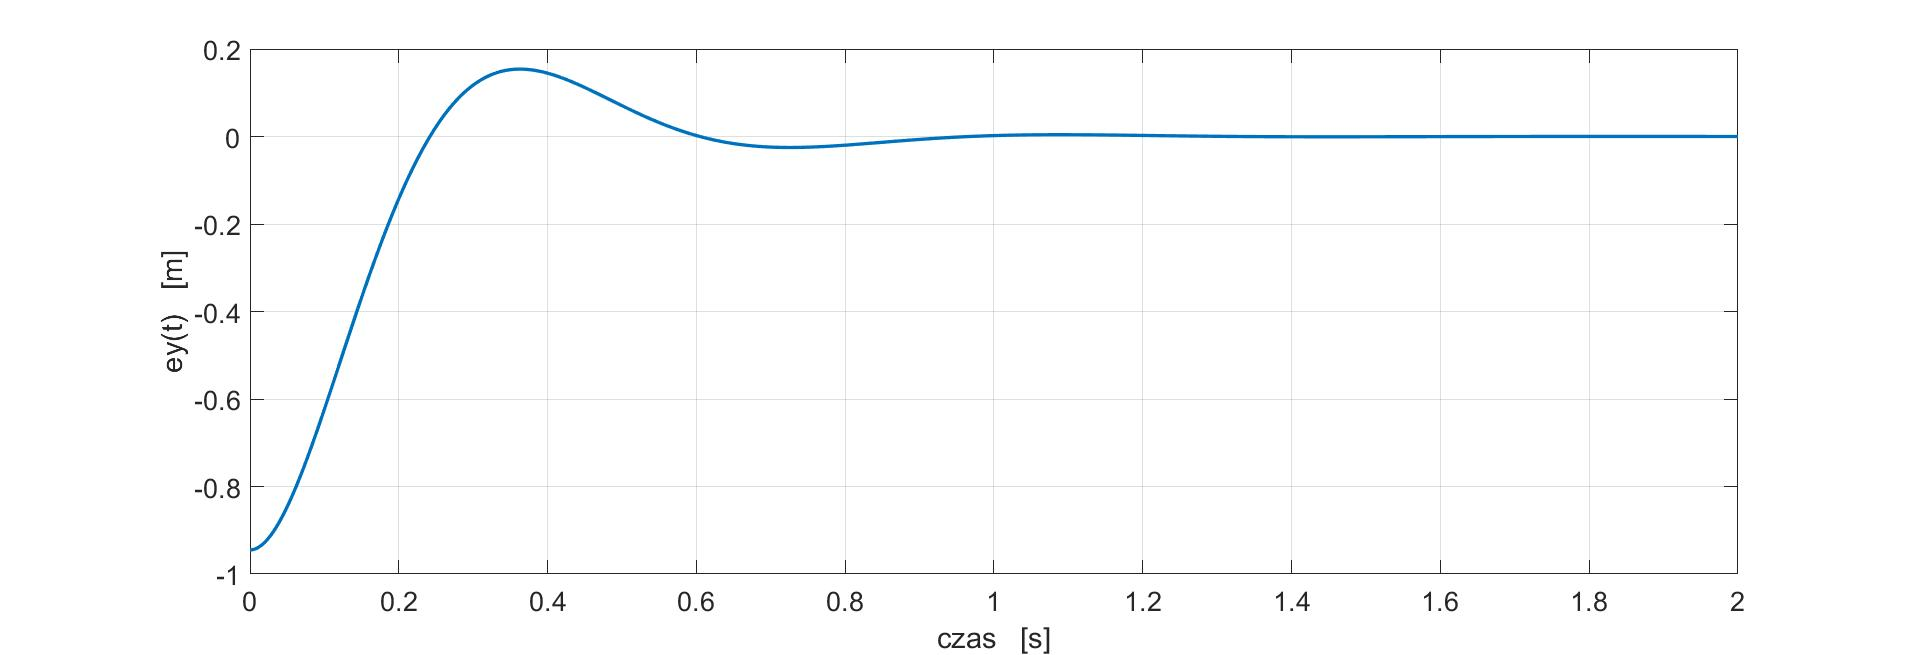
\includegraphics[width=1\textwidth]{eyodz.jpg}
\caption{\label{eyodz}Przebieg błędu $e_y(t)$ dla linii prostej wzdłuż osi OZ.}
\end{figure}
\begin{figure}[!h]
\centering
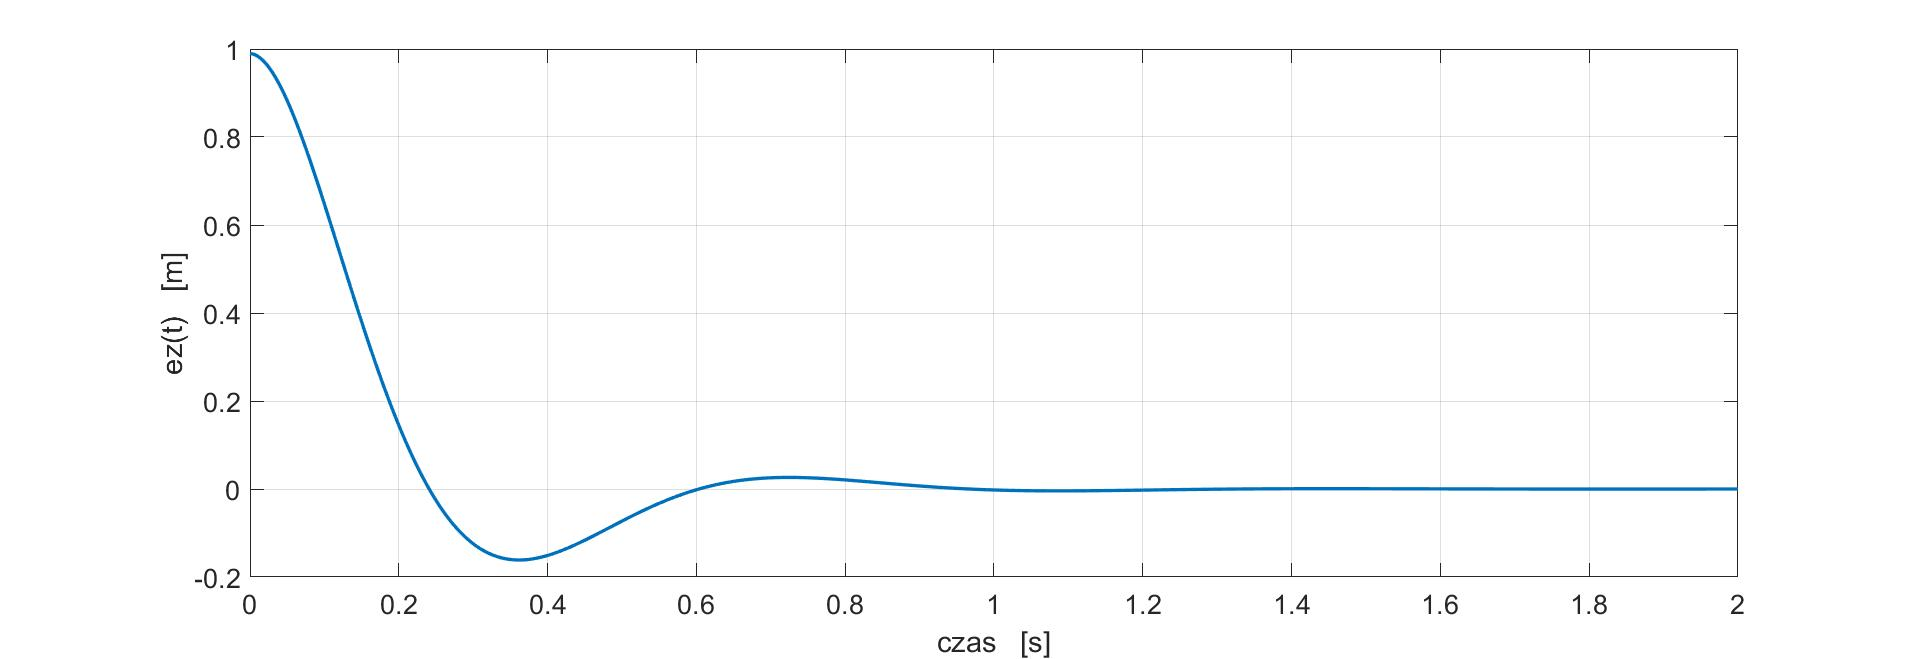
\includegraphics[width=1\textwidth]{ezodz.jpg}
\caption{\label{ezodz}Przebieg błędu $e_z(t)$ dla linii prostej wzdłuż osi OZ.}
\end{figure}
\newpage




\section{Ruch po trajektorii w kształcie kwadratu}
Wraz z opanowaniem sterowania po liniach prostych, można przystąpić do trajektorii efektora składających się z kilku odcinków. Prostym przykładem takiego ruchu jest ruch efektora po trajektorii o kształcie kwadratu. Ruch ten będzie wykonywany na płaszczyźnie $XY$ dla wartości $z=0$. Efektor ma rozpocząć swój ruch z punktu $L_0=(0.64; -0.94; 0)$. Następnie nakreśli kształt kwadratu o boku $50 $ cm. Zaprogramowanie takiego ruchu w Rapid dla np. manipulatora IRb-1400 wymagałoby użycia polecenia $MoveL$. Wymusza ta funkcja ruch efektora manipulatora po linii prostej do danego punktu. Przykłady fragment kodu


\begin{lstlisting}[frame=single] 
MoveL p1, v1000\T:=5, fine, tool0;
MoveL p2, v1000\T:=5, fine, tool0;
MoveL p3, v1000\T:=5, fine, tool0;
MoveL p4, v1000\T:=5, fine, tool0;
\end{lstlisting}
gdzie każemy wykonywać manipulatorowi ruchy efektorem po punktach $p1$, $p2$, $p3$, $p4$ w ciągu 20 sekund.

Wyniki pomiaru zależności współrzędnych położenia efektora w przestrzeni roboczej od czasu przedstawiono na wykresach \ref{kwx} oraz \ref{kwy}. Z kolei zależność współrzędnej $y$ od współrzędnej $x$, zarówno dla trajektorii zadanej jak i trajektorii rzeczywistej pokazano na rysunku \ref{kwxy}.
\hfill \break
\begin{figure}[!h]
\centering
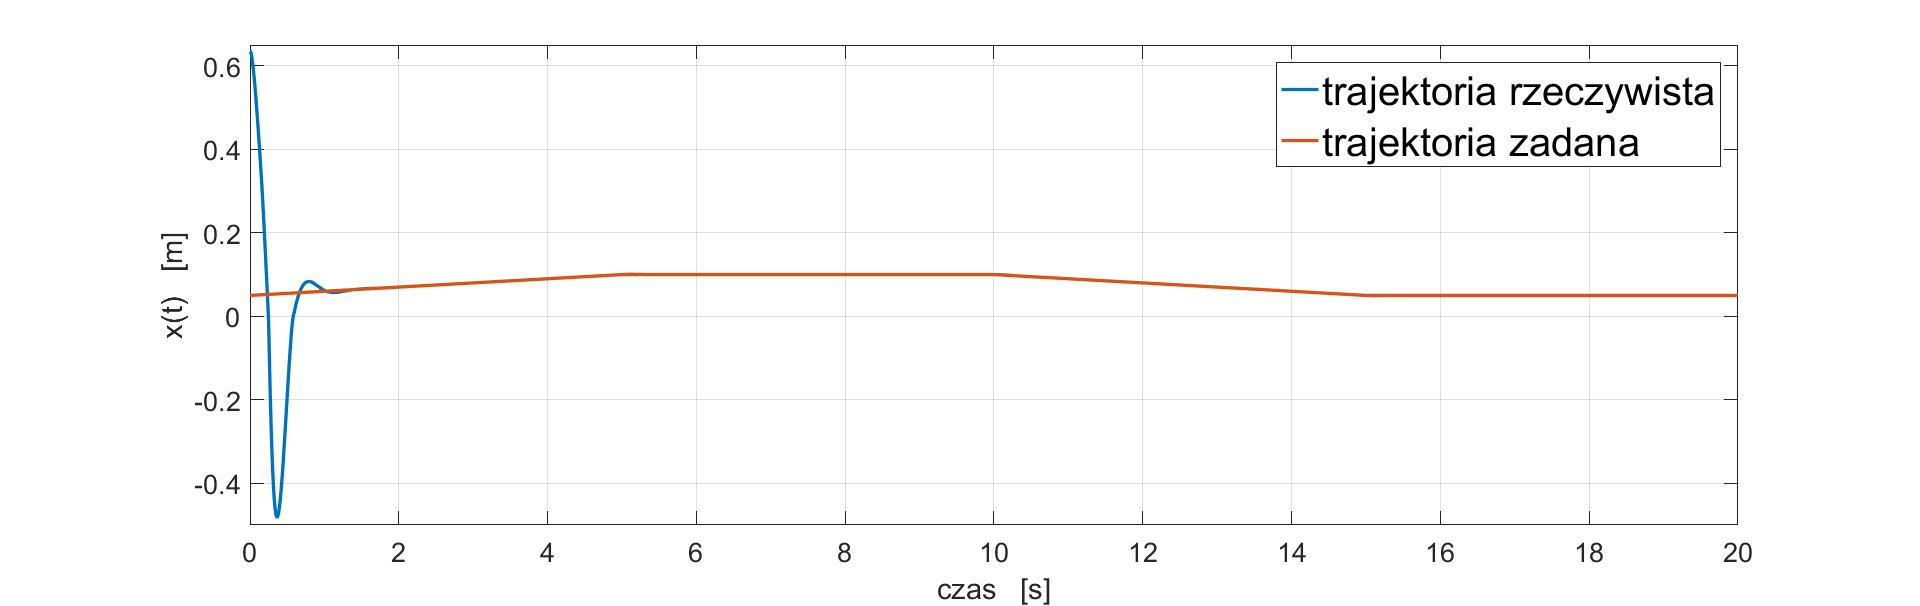
\includegraphics[width=1\textwidth]{kwx.jpg}
\caption{\label{kwx}Przebieg zmiennej $z(t)$ dla trajektorii zadanej oraz rzeczywistej.}
\end{figure}
\begin{figure}[!h]
\centering
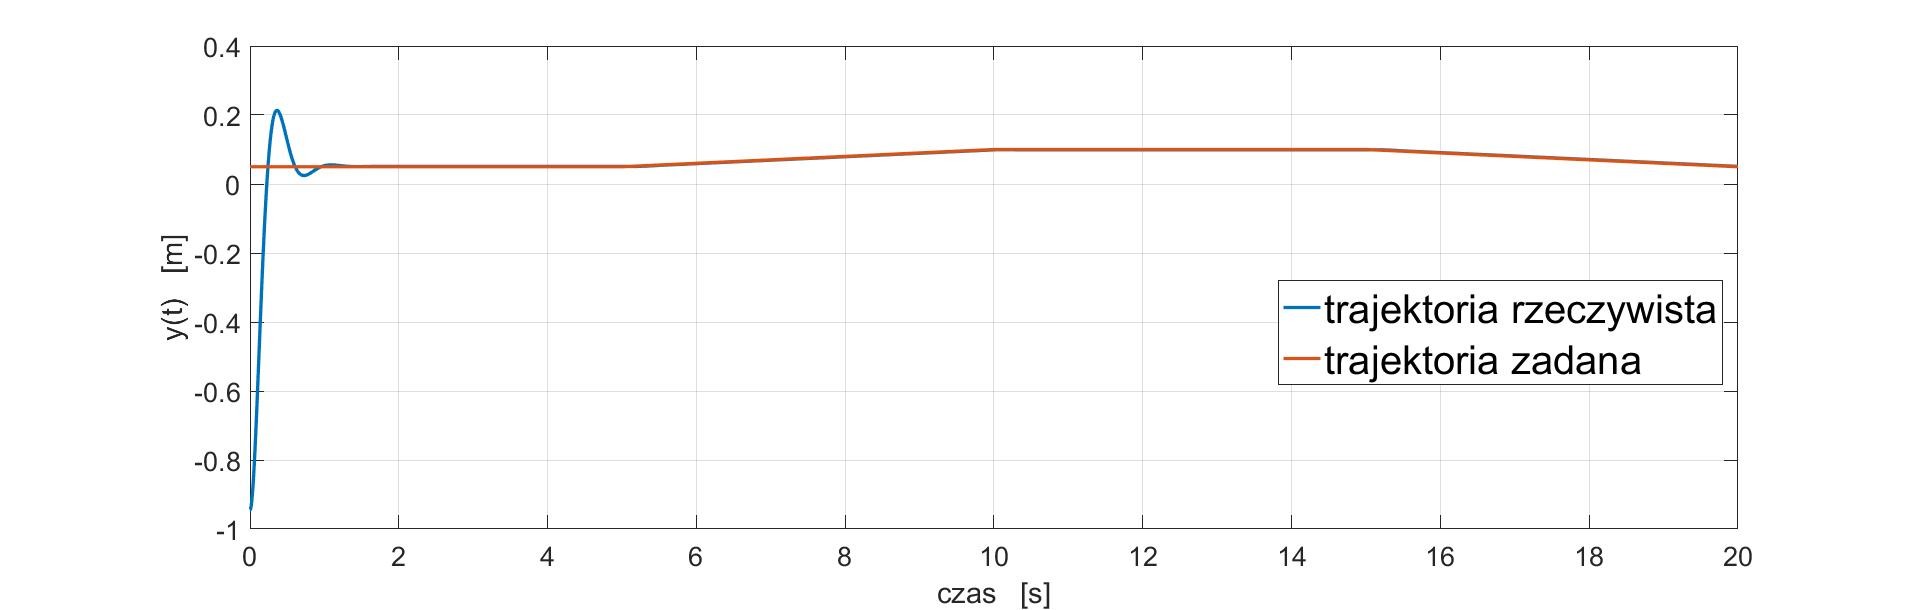
\includegraphics[width=1\textwidth]{kwy.jpg}
\caption{\label{kwy}Sygnały sterujące $u(t)$ dla ruchu po linii prostej w kierunku osi OZ.}
\end{figure}
\begin{figure}[!h]
\centering
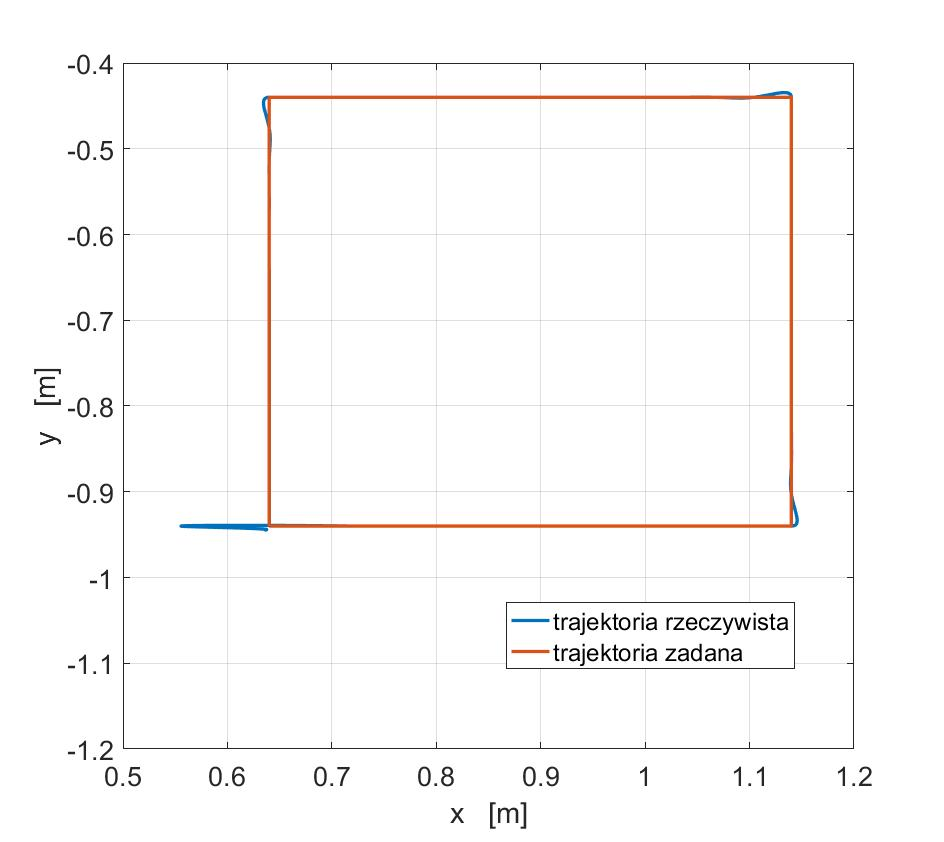
\includegraphics[width=1\textwidth]{kwxy.jpg}
\caption{\label{kwxy}Trajektorie efektora w przestrzeni XY.}
\end{figure}

Następnie zmierzono zależność uchybu sterowania dla ruchu po kwadracie. Wynikowe charakterystyki przedstawiono na wykresach \ref{exkw}, \ref{eykw} oraz \ref{ezkw}.
\hfill \break
\begin{figure}[!h]
\centering
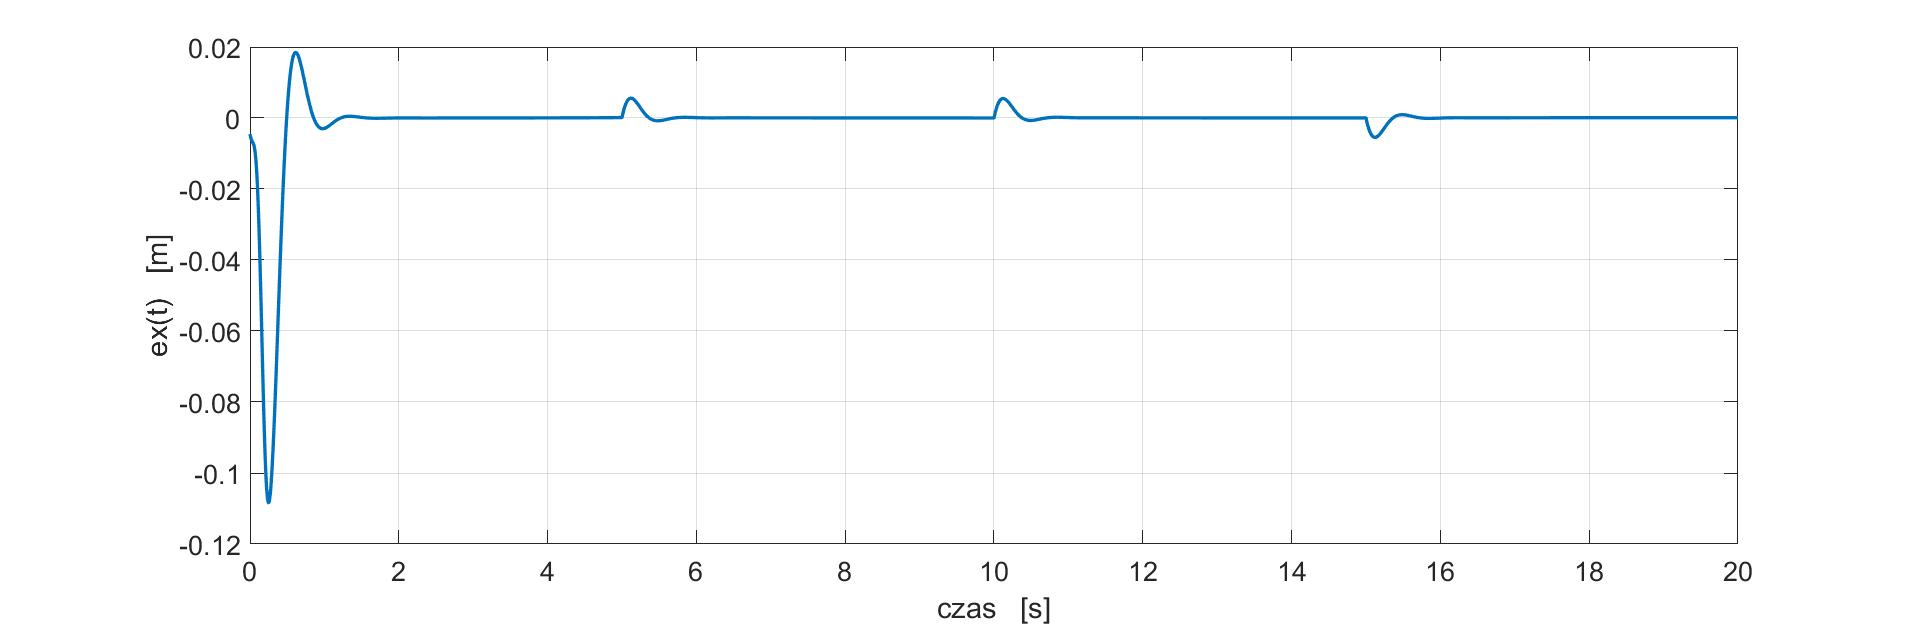
\includegraphics[width=1\textwidth]{exkw.jpg}
\caption{\label{exkw}Przebieg błędu $e_x(t)$ dla ruchu po kwadracie.}
\end{figure}
\begin{figure}[!h]
\centering
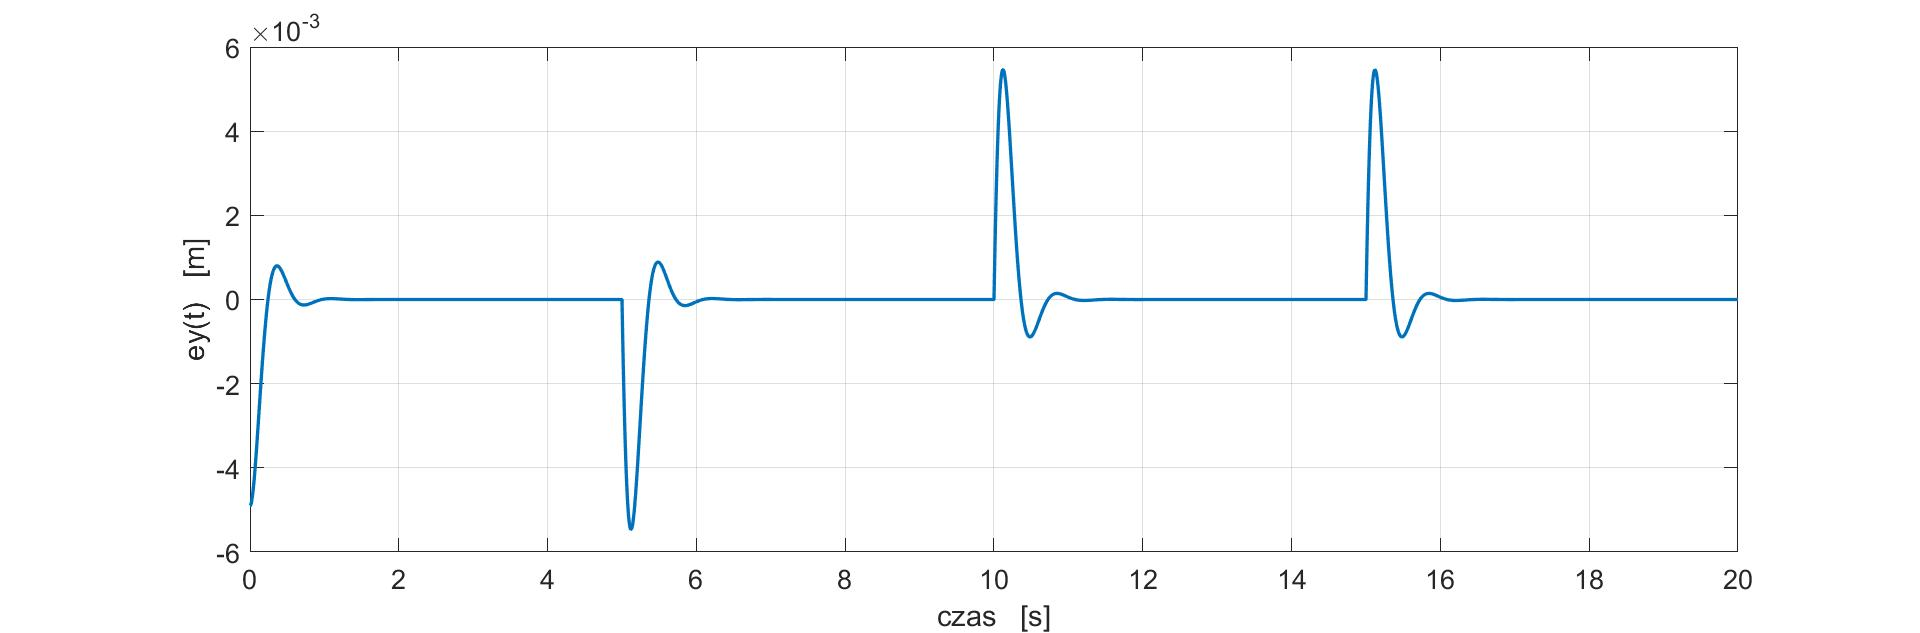
\includegraphics[width=1\textwidth]{eykw.jpg}
\caption{\label{eykw}Przebieg błędu $e_y(t)$ dla ruchu po kwadracie.}
\end{figure}
\begin{figure}[!h]
\centering
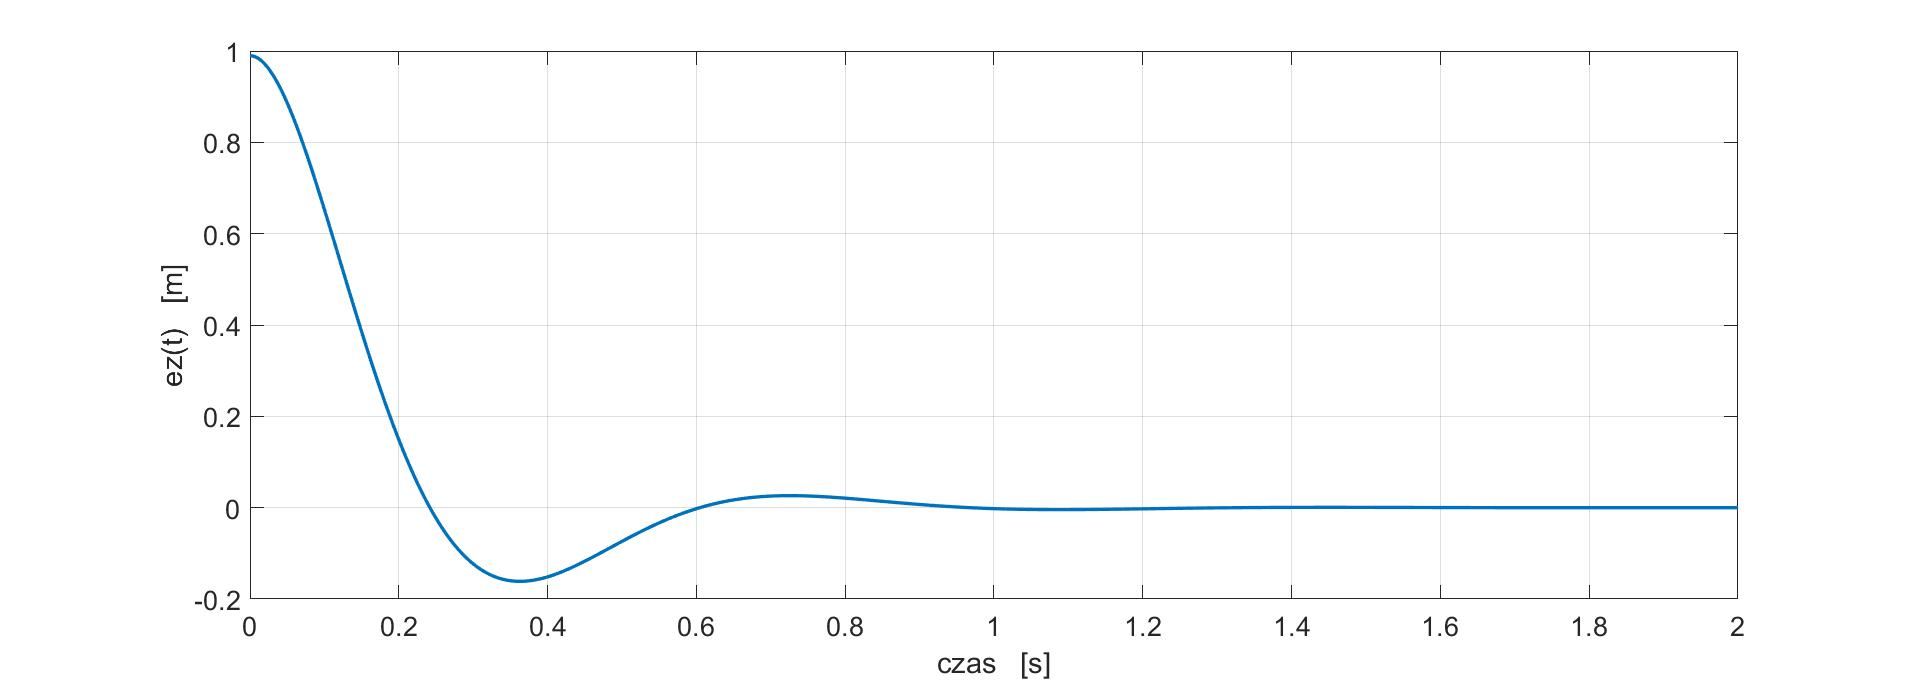
\includegraphics[width=1\textwidth]{ezkw.jpg}
\caption{\label{ezkw}Przebieg błędu $e_z(t)$ dla ruchu po kwadracie.}
\end{figure}













\newpage
\newpage
\section{Ruch śrubowy}
Ostatecznym celem zbadania skuteczności algorytmu odsprzęgania wejściowo-wyjściowego miało być poprowadzenie efektora ruchem śrubowym określonej układem równań (\ref{row4.1}). Zależność współrzędnych trajektorii zarówno zadanej jak i rzeczywistej przedstawiono na wykresach \ref{srubx}, \ref{sruby} oraz \ref{srubz}.
\hfill \break
\begin{figure}[!h]
\centering
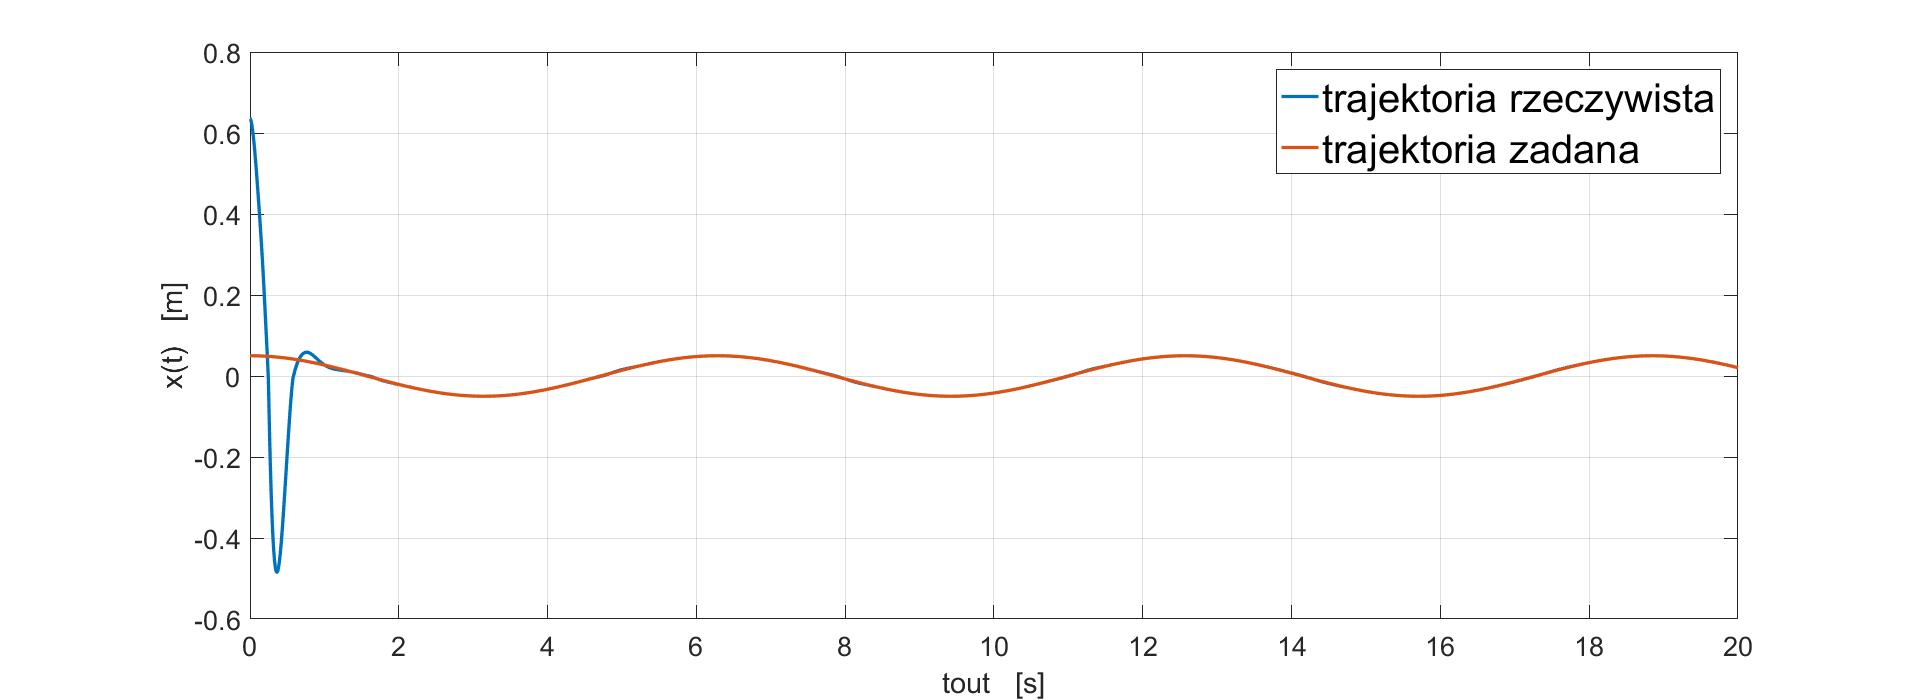
\includegraphics[width=1\textwidth]{srubx.jpg}
\caption{\label{srubx}Przebieg zmiennej $x(t)$ ruchu śrubowego dla trajektorii zadanej oraz rzeczywistej.}
\end{figure}
\begin{figure}[!h]
\centering
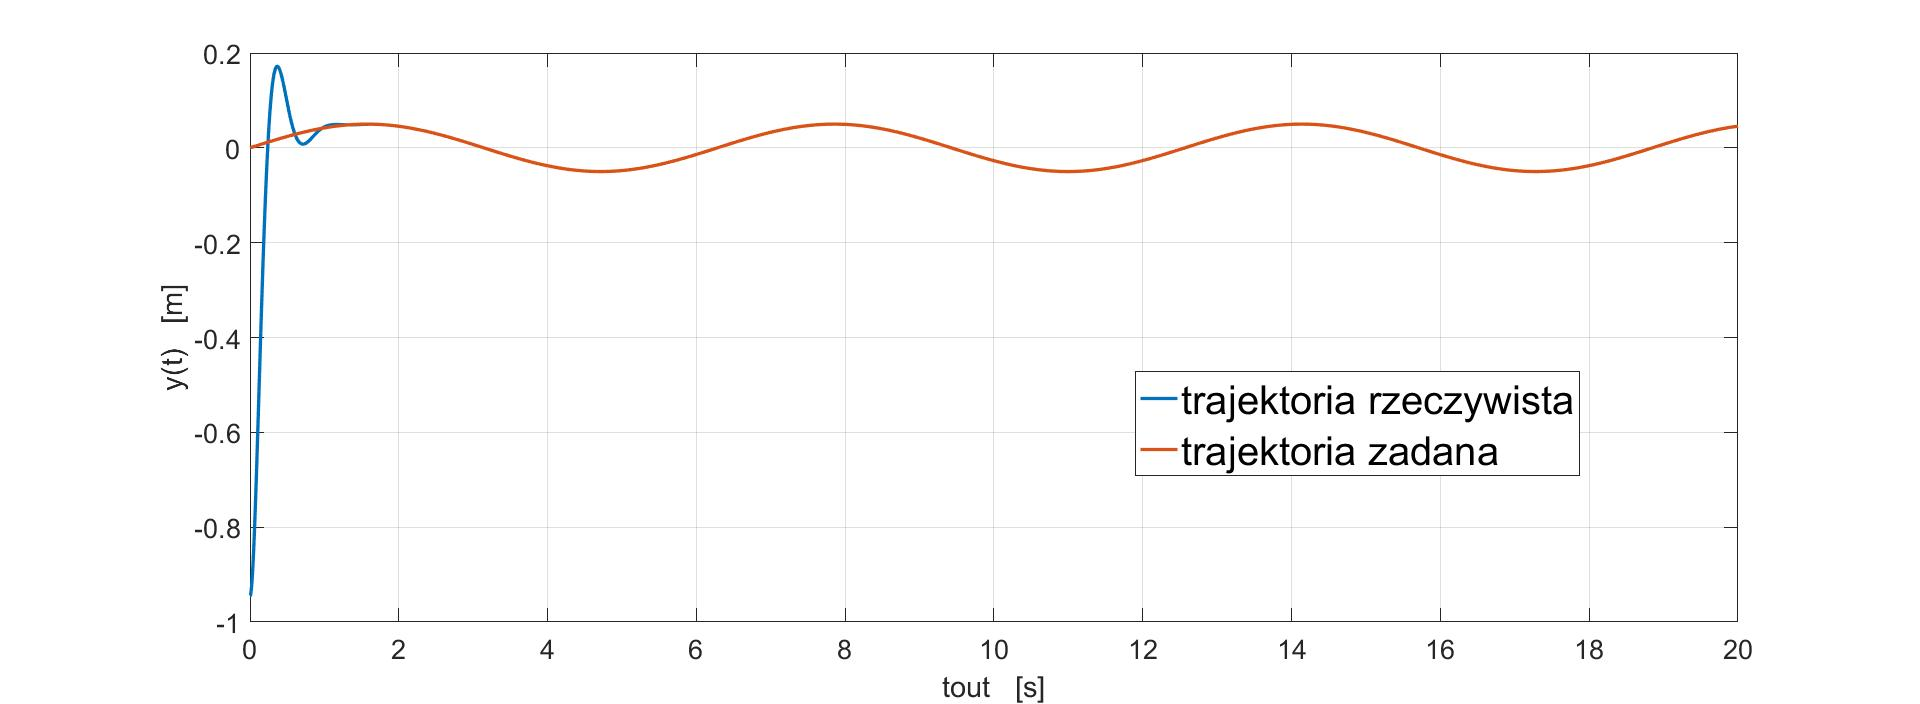
\includegraphics[width=1\textwidth]{sruby.jpg}
\caption{\label{sruby}Przebieg zmiennej $y(t)$ ruchu śrubowego dla trajektorii zadanej oraz rzeczywistej.}
\end{figure}
\begin{figure}[!h]
\centering
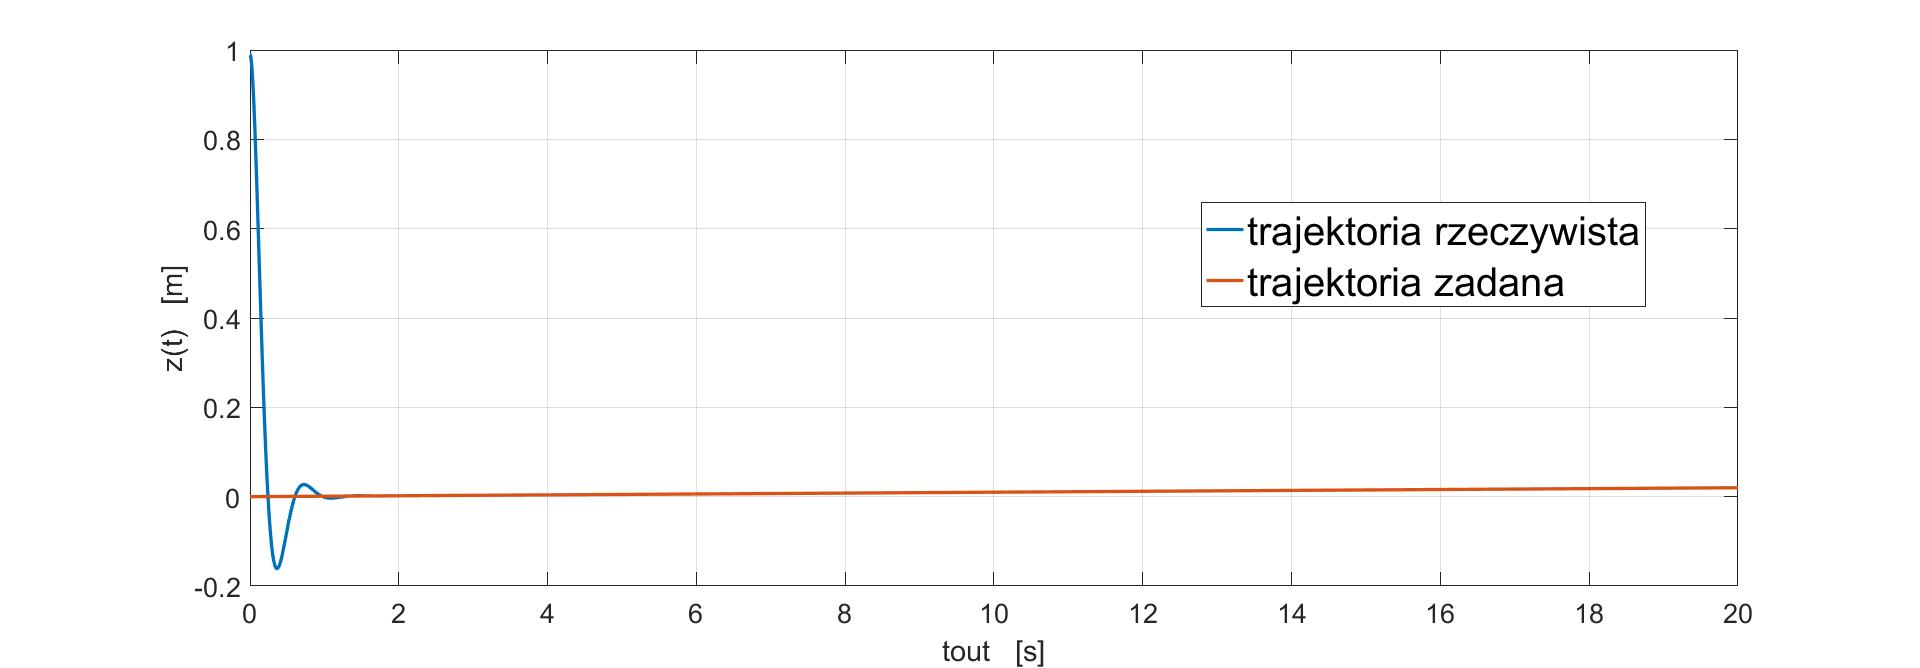
\includegraphics[width=1\textwidth]{srubz.jpg}
\caption{\label{srubz}Przebieg zmiennej $z(t)$ ruchu śrubowego dla trajektorii zadanej oraz rzeczywistej.}
\end{figure}

W celu dobrej wizualizacji sterowania efektorem dla tej trajektorii, zastosowano trójwymiarowy wykres \ref{srubxyz}. Odzwierciedla on dobrze trajektorię ruchu chwytaka w przestrzeni roboczej. 
\begin{figure}[!h]
\centering
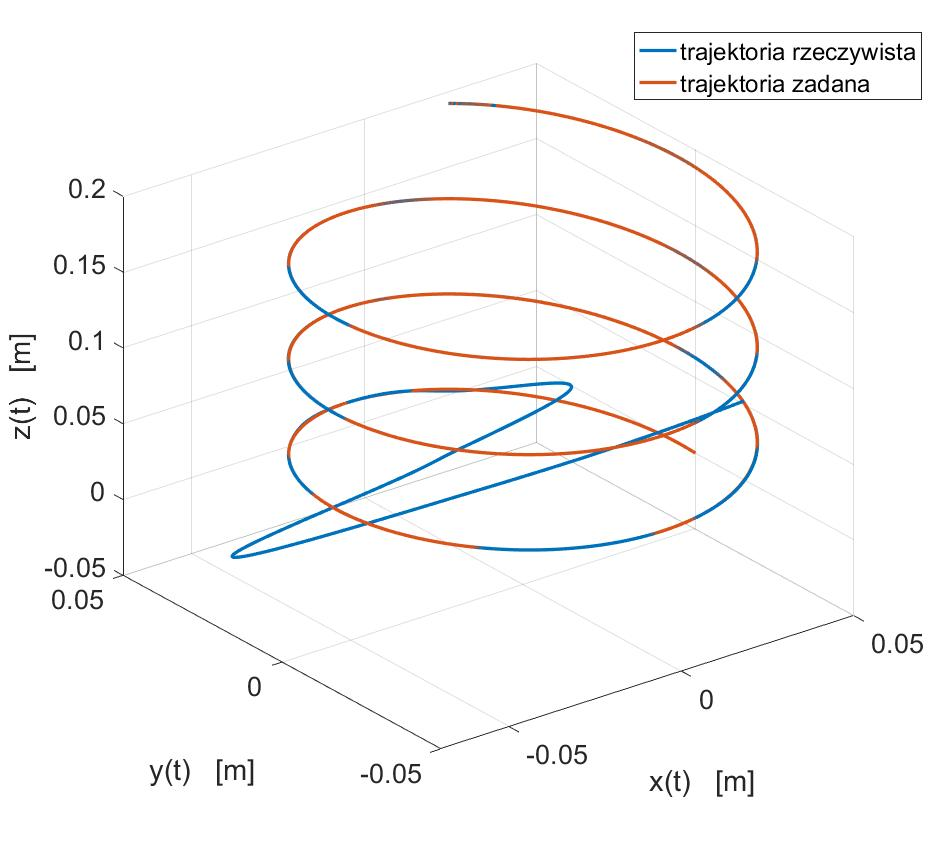
\includegraphics[width=1\textwidth]{srubxyzv2.jpg}
\caption{\label{srubxyz}Trajektoria chwytaka w przestrzeni XYZ dla ruchu śrubowego.}
\end{figure}
\chapter{Podsumowanie}
W pracy stworzono model manipulatora IRb-6, w środowisku Matlab/Simulink. Bazując na bibliografii opisano dokładnie jego dynamikę oraz kinematykę, które miały być podstawą do przeprowadzenia symulacji. 

Następnie zrealizowano implementację algorytmu odsprzęgania wejściowo-wyjściowego. Pomyślnie stworzono afiniczny układ sterowania. Jednocześnie dla tego układu wyliczono konfiguracje osobliwe, których unikano w sterowaniu na etapie badań symulacyjnych. Gdy udało się zaimplementować sterowanie odsprzęgające i linearyzujące, utworzono w środowisku symulacyjnym generator trajektorii zadanej oraz regulację PD. 

Na podstawie tak prawidłowo utworzonego sterowania z regulacją przeprowadzono badania symulacyjne. Przebadano ruch prostoliniowy w kierunku poszczególnych osi OX, OY oraz OZ. Potem sprawdzono skuteczność sterowania dla ruchu po kwadracie na płaszczyźnie XY. Na końcu dokonano symulacji ruchu efektora po trajektorii śruby. Za każdym razem sprawdzano czy manipulator nie znajduje się w konfiguracji osobliwej. 

Manipulator wykonywał odpowiednio wszystkie zadanie trajektorie. Wszystkie badane przebiegi uchybu dążyły do zera. Większe początkowe wartości uchybów często wynikały z oddalenia początkowego położenia efektora od trajektorii zadanej. Jednak różnica ta była szybko niwelowana. W ruchu efektora po kwadracie można zaobserwować lekkie wzrosty wartości uchybów przy każdej nagłej zmianie kierunku poruszania się chwytaka. Wynikają one jednak ze skokowych zmian wartości sygnałów sterowania. W trakcie pozostałego czasu wykonywania tej trajektorii przez manipulator uchyb utrzymywał wartość zero. Pomyślnie zaimplementowano na modelu robota IRb-6 algorytm odsprzęgania wejściowo-wyjściowego. \bf{Cel pracy został zrealizowany}.







\addcontentsline{toc}{chapter}{Bibliografia} %utworzenie w spisie treści pozycji Bibliografia
\begin{thebibliography}{9}

\bibitem{b1}
  K. Tchoń, A. Mazur, I. Dulęba, R. Hossa, R. Muszyński
  \emph{Manipulatory i roboty mobilne. Modele, planowanie ruchu, sterowanie}.
  Akademicka Oficyna Wydawnicza PLJ, Warszawa,
  2000.
\bibitem{b2}
M. Spong, S. Hutchinson, M. Vidyasagar, 
\emph{Dynamika i sterowanie robotów}.
WNT, Warszawa,1997.
\bibitem{b3}
A. Isidori, \emph{Nonlinear Control Systems}.
Springer, Londyn, 1995.
\bibitem{b4}
A. Gosiewski i in., 
\emph{Badanie własnosci dynamicznych oraz projekt regulacji nadążnej dla robotów IRb-6 oraz IRb-60}.
Raport IA Politechniki Warszawskiej, Warszawa, 1984.
\bibitem{b5}
T. Szkodny, \emph{Modelowanie i symulacja ruchu manipulatorów robotów przemysłowych}. 
Wydawnictwo Politechniki Śląskiej, Gliwice, 2004.
\end{thebibliography}



\end{document}